%%%%%%%%%%%%%%%%%%%%%%%%%%%%%%%%%%%%%%%%%%  不使用 authblk 包制作标题  %%%%%%%%%%%%%%%%%%%%%%%%%%%%%%%%%%%%%%%%%%%%%%
%-------------------------------PPT Title-------------------------------------
\title{04-固体能带理论}
%-----------------------------------------------------------------------------

%----------------------------Author & Date------------------------------------
%\author[\textrm{Jun\_Jiang}]{姜\;\;骏\inst{}} %[]{} (optional, use only with lots of authors)
%% - Give the names in the same order as the appear in the paper.
%% - Use the \inst{?} command only if the authors have different
%%   affiliation.
%\institute[BCC]{\inst{}%
\institute[Gain~Strong]{\inst{}%
%\vskip -20pt 北京市计算中心}
\vskip -20pt {\large 格致斯创~科技}}
\date[\today] % (optional, should be abbreviation of conference name)
{%	{\fontsize{6.2pt}{4.2pt}\selectfont{\textcolor{blue}{E-mail:~}\url{jiangjun@bcc.ac.cn}}}
\vskip 45 pt {\fontsize{8.2pt}{6.2pt}\selectfont{%清华大学\;\;物理系% 报告地点
	\vskip 5 pt \textrm{2022.11.26}}}
}

%% - Either use conference name or its abbreviation
%% - Not really information to the audience, more for people (including
%%   yourself) who are reading the slides onlin%%   yourself) who are reading the slides onlin%%   yourself) who are reading the slides onlineee
%%%%%%%%%%%%%%%%%%%%%%%%%%%%%%%%%%%%%%%%%%%%%%%%%%%%%%%%%%%%%%%%%%%%%%%%%%%%%%%%%%%%%%%%%%%%%%%%%%%%%%%%%%%%%%%%%%%%%

\subject{}
\small
\frame
{
	\frametitle{\rm{DFT}之歌}
\begin{figure}[h!]
	\vspace{-10pt}
\centering
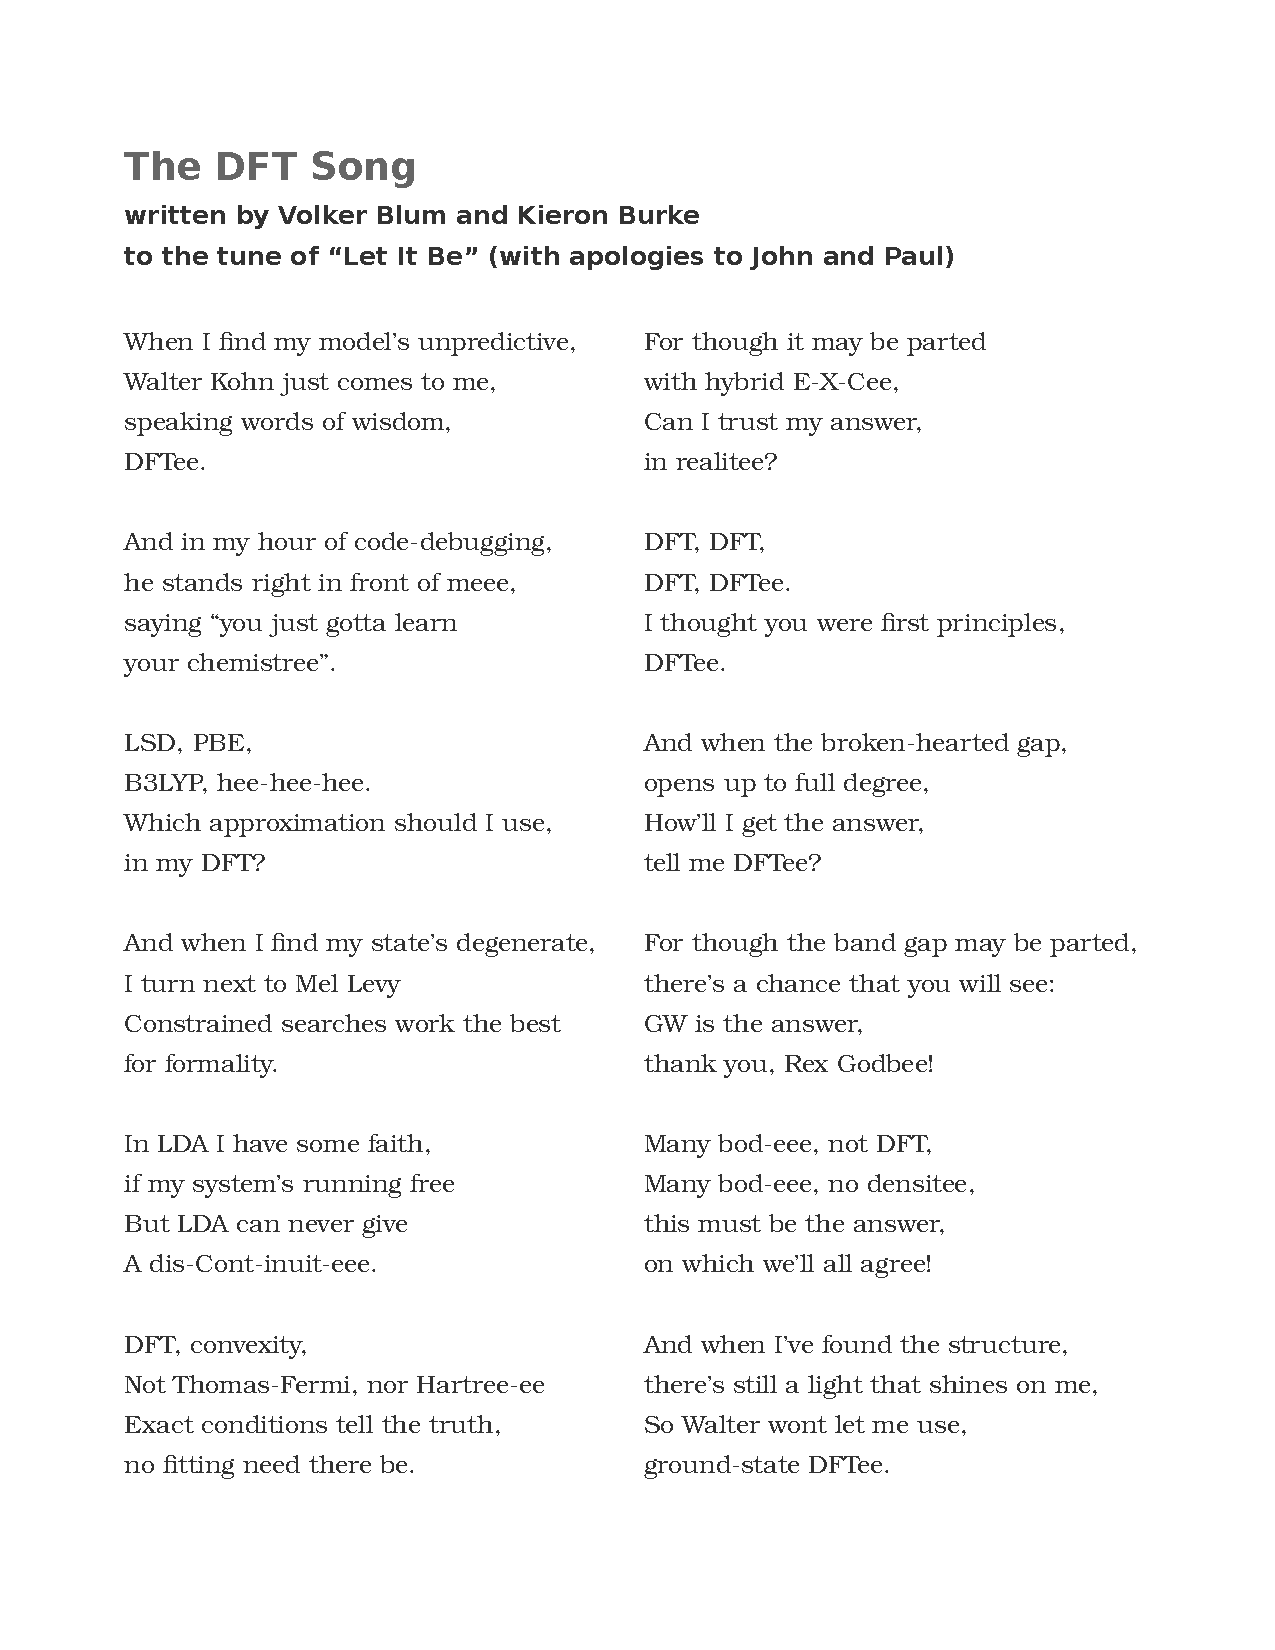
\includegraphics[height=2.85in,width=3.8in,viewport=0 350 550 720,clip]{Figures/DFT_song-1.pdf}
%\caption{\tiny \textrm{The Nolbel Prize in Chemistry 1998 Summary.}}%(与文献\cite{EPJB33-47_2003}图1对比)
\label{DFT_Song_01}
\end{figure}
}

\frame
{
	\frametitle{}
\begin{figure}[h!]
	\vspace{-10pt}
\centering
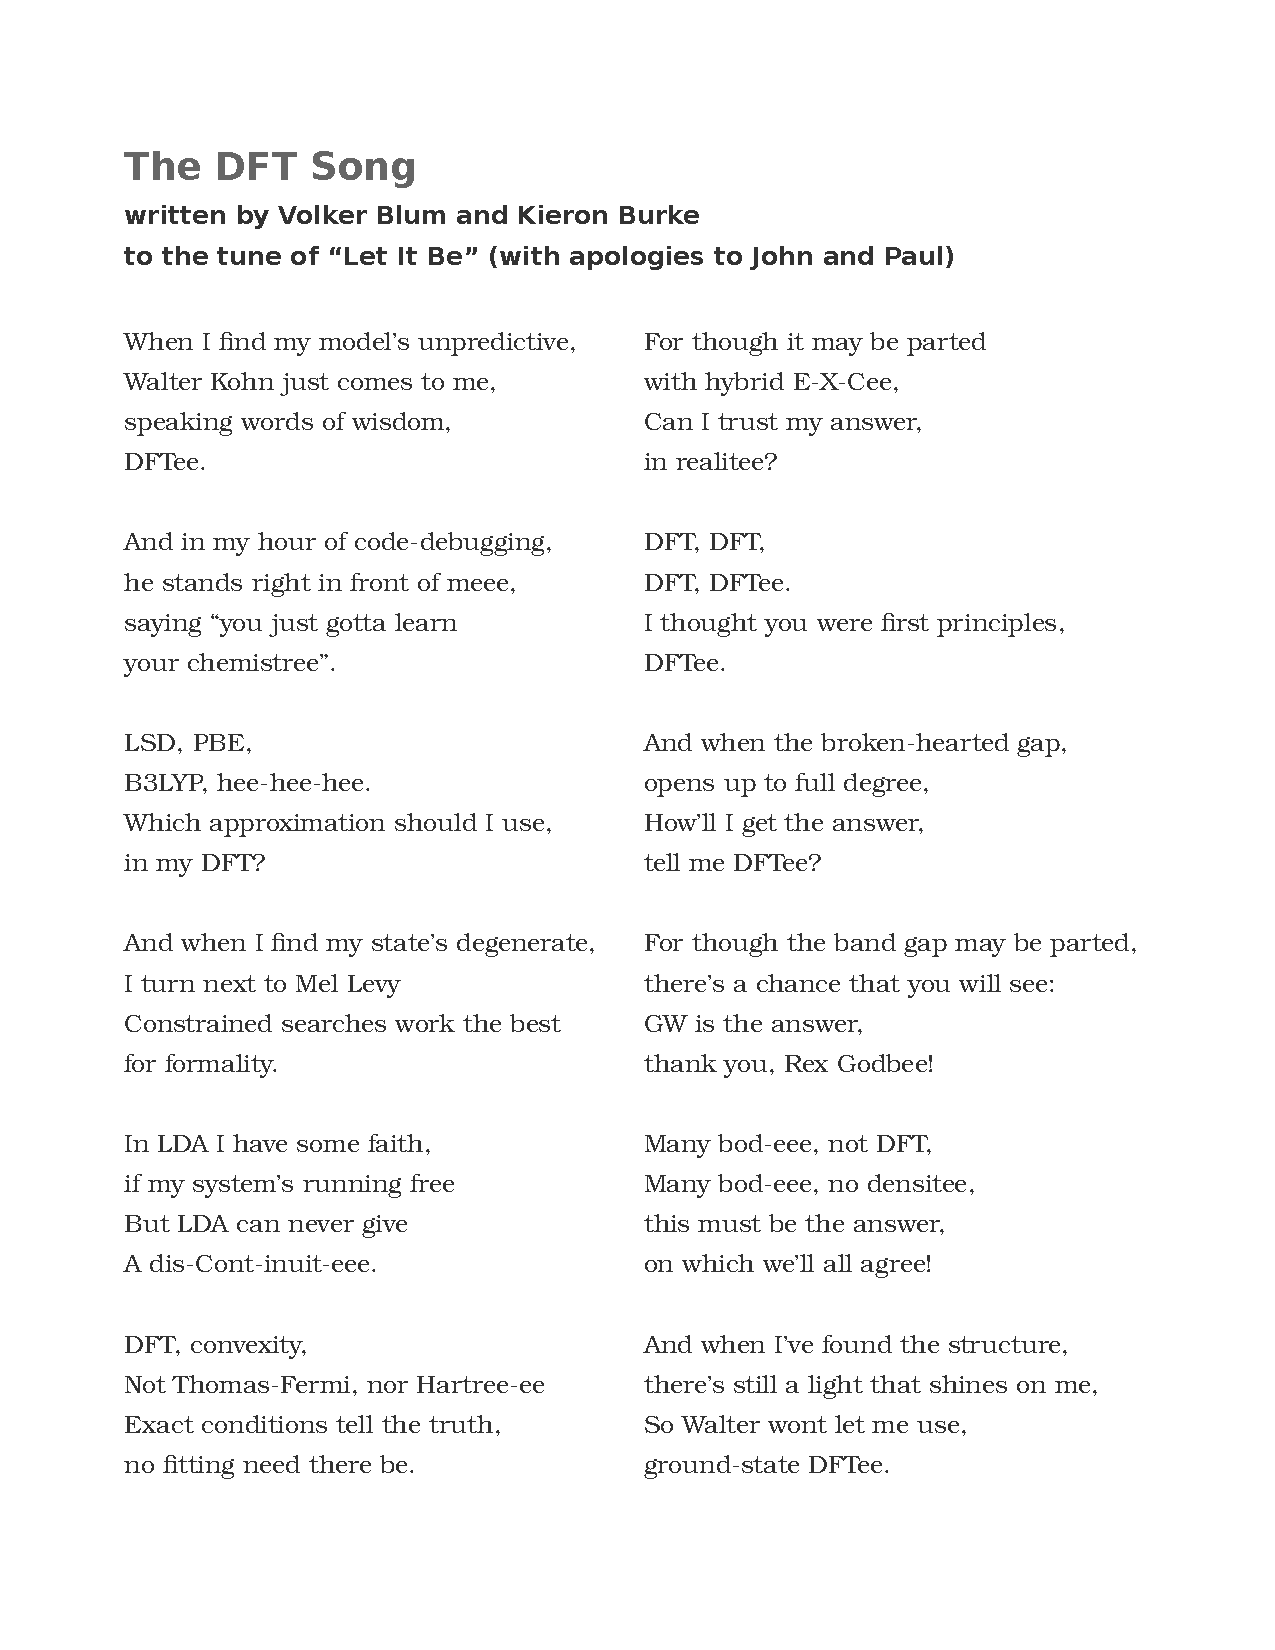
\includegraphics[height=1.95in,width=3.8in,viewport=0 80 550 352,clip]{Figures/DFT_song-1.pdf}
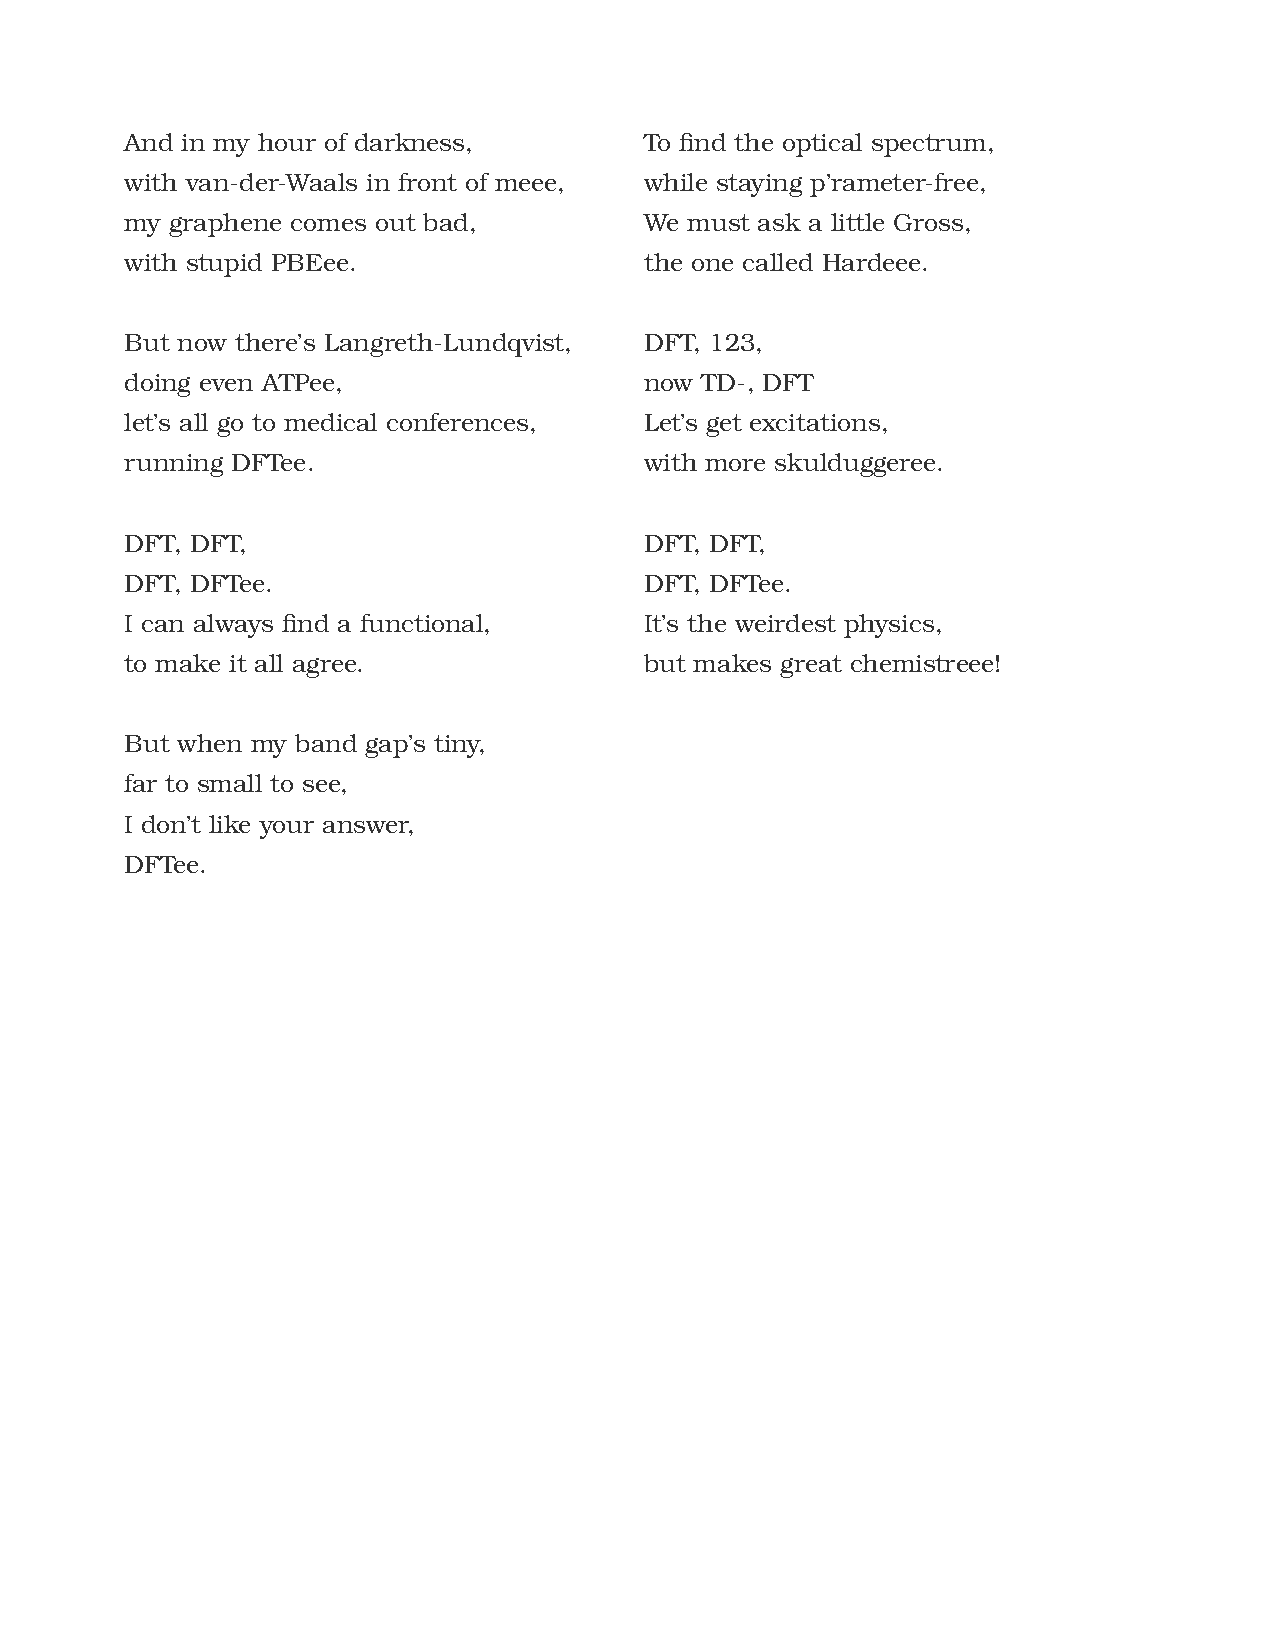
\includegraphics[height=0.70in,width=3.8in,viewport=0 650 550 750,clip]{Figures/DFT_song-2.pdf}
%\caption{\tiny \textrm{The Nolbel Prize in Chemistry 1998 Summary.}}%(与文献\cite{EPJB33-47_2003}图1对比)
\label{DFT_Song_02}
\end{figure}
}

\frame
{
	\frametitle{}
\begin{figure}[h!]
	\vspace{-10pt}
\centering
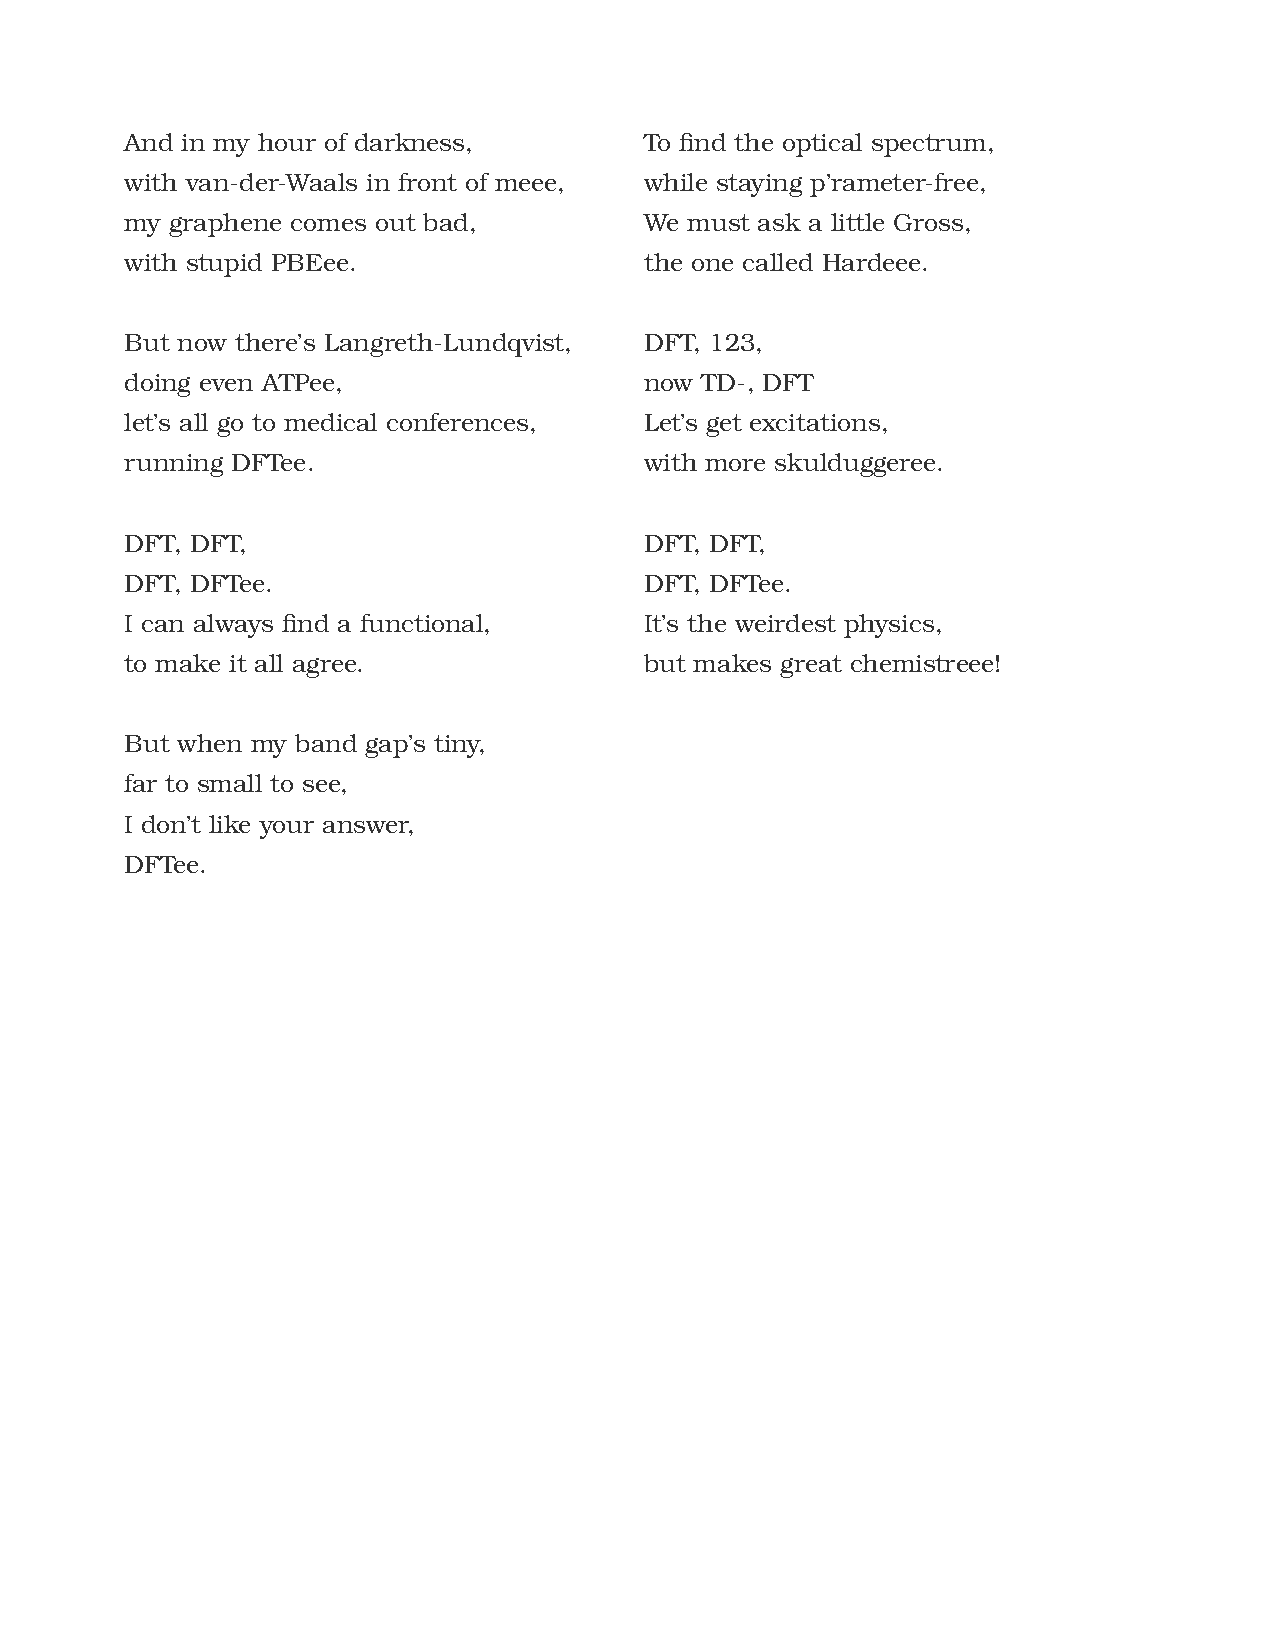
\includegraphics[height=2.10in,width=3.8in,viewport=0 350 550 650,clip]{Figures/DFT_song-2.pdf}
%\caption{\tiny \textrm{The Nolbel Prize in Chemistry 1998 Summary.}}%(与文献\cite{EPJB33-47_2003}图1对比)
\includemovie[poster, controls, mouse, url] {0.8\textwidth}{0.1\textwidth}{Figures/DFT_Song.mp3}     %
%\includemovie[poster, controls, mouse, url] {0.8\textwidth}{0.2\textwidth}{Figures/DFT_Song_accompany.mp3}     %
\label{DFT_Song_03}
\end{figure}
}

% This is only inserted into the PDF information catalog. Can be left
% out.
%\maketitle
\frame
{
%	\frametitle{\fontsize{9.5pt}{5.2pt}\selectfont{\textcolor{orange}{“高通量并发式材料计算算法与软件”年度检查}}}
\titlepage
}
%-----------------------------------------------------------------------------

%------------------------------------------------------------------------------列出全文 outline ---------------------------------------------------------------------------------
%\section*{}
%\frame[allowframebreaks]
%{
%  \frametitle{Outline}
%%  \frametitle{\textcolor{mycolor}{\secname}}
%  \tableofcontents%[current,currentsection,currentsubsection]
%}
%%在每个section之前列出全部Outline
%%类似的在每个subsection之前列出全部Outline是\AtBeginSubsection[]
%\AtBeginSection[]
%{
%  \frame<handout:0>%[allowframebreaks]
%  {
%    \frametitle{Outline}
%%全部Outline中,本部分加亮
%    \tableofcontents[current,currentsection]
%  }
%}

%-----------------------------------------------PPT main Body------------------------------------------------------------------------------------
\small
\section{固体能带理论}       %Bookmark
\frame
{
%\frametitle{The Bloch theorem}
	\frametitle{\textrm{Bloch~}定理}
\begin{itemize}%[+-| alert@+>]
   \setlength{\itemsep}{8pt}
   \item 固体能带理论\upcite{Huang-Han}是固体电子理论的基础,形式上是单电子理论:
    $$\hat H |\psi_i^{\vec k}(\vec r)\rangle=\bigg[-\dfrac{\hbar^2}{2m}\nabla^2+V(\vec r)\bigg]|\psi_i^{\vec k}(\vec r)\rangle=\epsilon_i(\vec k)|\psi_i^{\vec k}(\vec r)\rangle$$
  \item \textrm{Bloch}定理:
%   \item \textrm{periodic potential:} $$V(\vec r)=V(\vec r+\vec R_n)$$
%     \textrm{Here,} $\vec R_n=n\vec R$
%   \item \textrm{Bloch theorem:}$$\psi_{\vec k}(\vec r)=\textrm{e}^{\textrm i\vec k\cdot\vec r}u_{\vec k}(\vec r)$$
%     \textrm{Here, $u_{\vec k}(\vec r)$ is a periodic function with the same periodicity as $V(\vec r)$, i.e., $u_{\vec k}(\vec r)=u_{\vec k}(\vec r+\vec R_n)$, then Bloch theorem could reads as:}
%     $$\psi_{\vec k}(\vec r+\vec R_n)=\textrm{e}^{\textrm i\vec k\cdot\vec R_n}\psi_{\vec k}(\vec r)$$
具有平移周期性的理想晶体,势能$V(\vec r)$满足$$V(\vec r)=V(\vec r+\vec R_n)$$
体系的波函数满足\textrm{Bloch}波函数形式:$$\psi_{\vec k}(\vec r)=\textrm{e}^{i\vec k\cdot\vec r}u_{\vec k}(\vec r)$$
是平面波和周期函数的乘积。$u(\vec r)$与势能有相同的周期。即$$u_{\vec k}(\vec r)=u_{\vec k}(\vec r+\vec R_n)$$
  \item 能带理论相当于分子轨道理论
%   \setlength{\itemsep}{30pt}
\item \textrm{Bloch}函数反映了波函数在周期性势场下的变化规律。
\end{itemize}
}

\frame
{
\frametitle{周期体系的波函数}
物质的电子体系,可分为芯层分子和价层电子。芯电子能量低,受周围化学环境影响很小,基本保持原子属性;价层电子相互作用较强,对化学环境较为敏感。一般地,价电子波函数在原子间区域(\textrm{Interstitial}区)的变化平缓,在临近原子核附近区域(\textrm{Muffin-tin}球内),会出现剧烈振荡(与芯层波函数正交)。
\begin{figure}[h!]
\centering
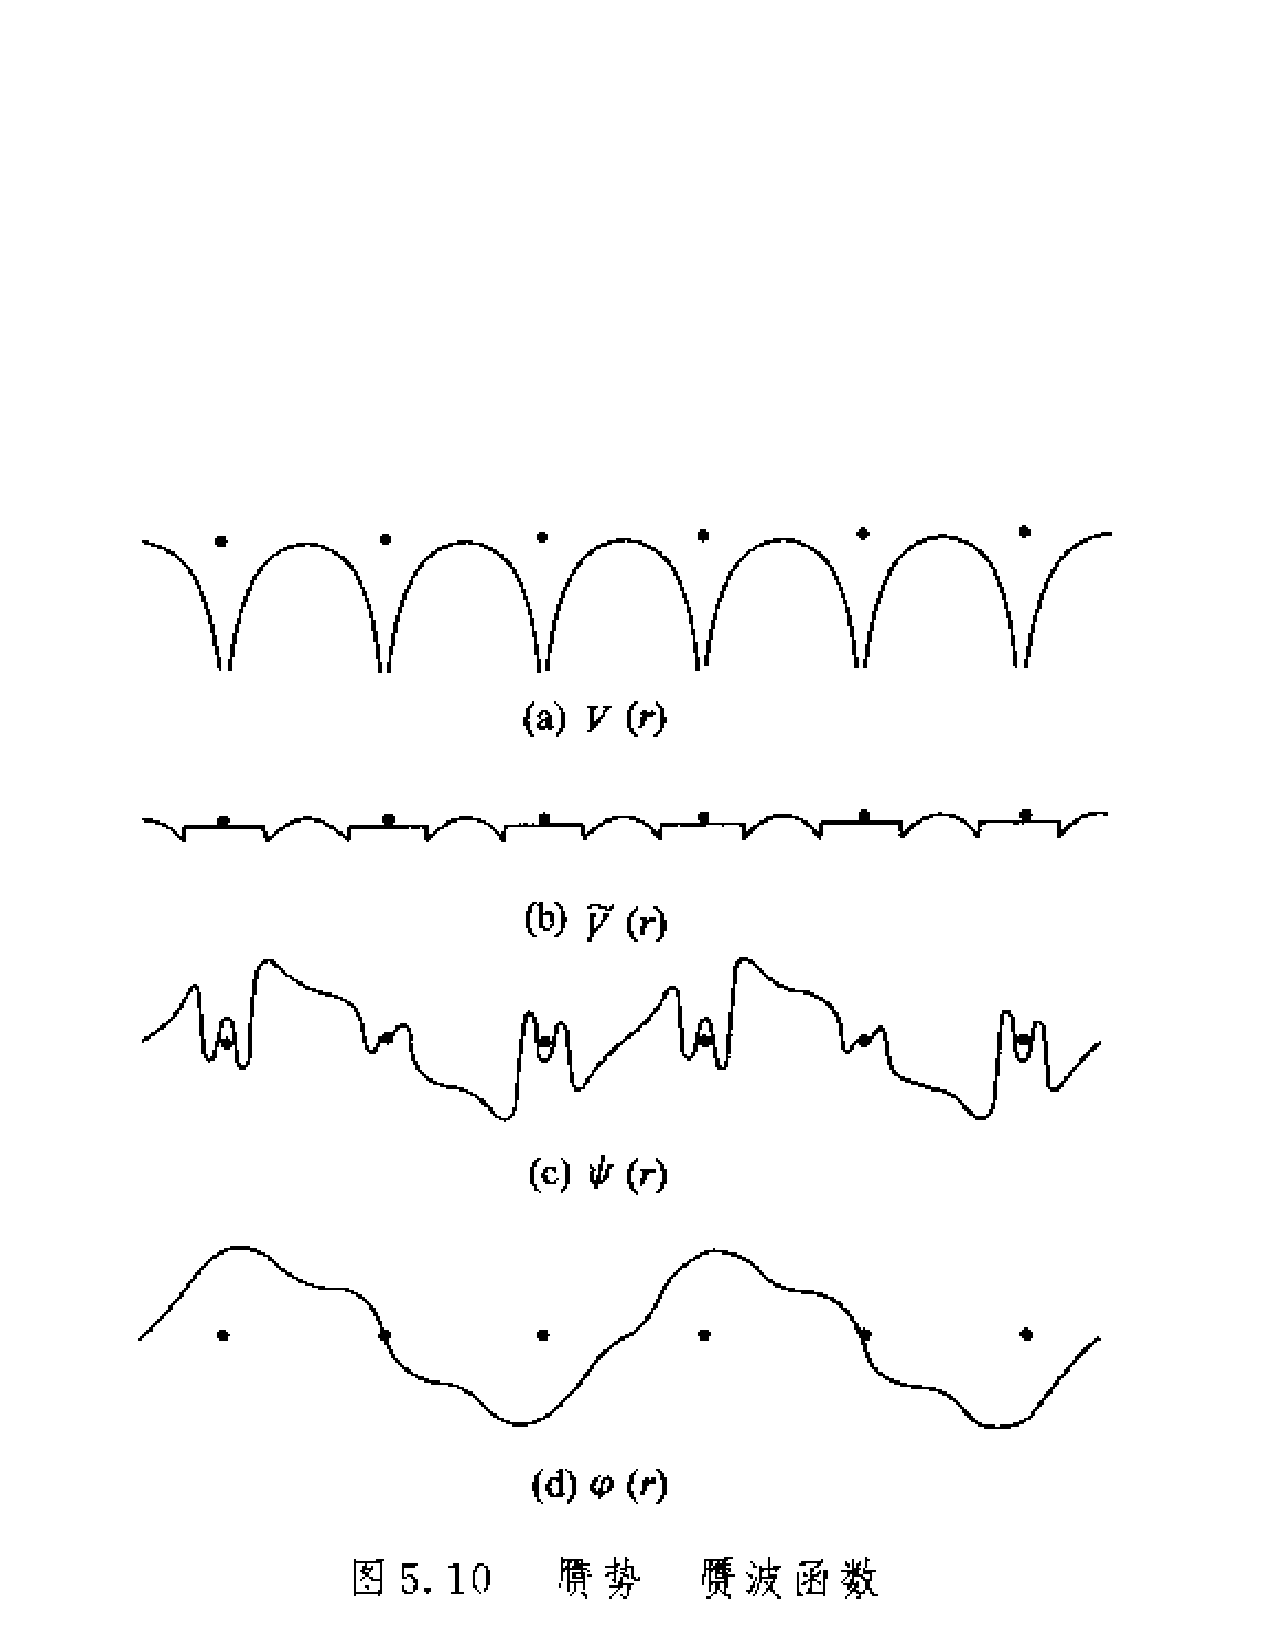
\includegraphics[height=0.8in,width=4.in,viewport=41 433 539 546,clip]{Figures/Pseudo_wave.pdf}\\
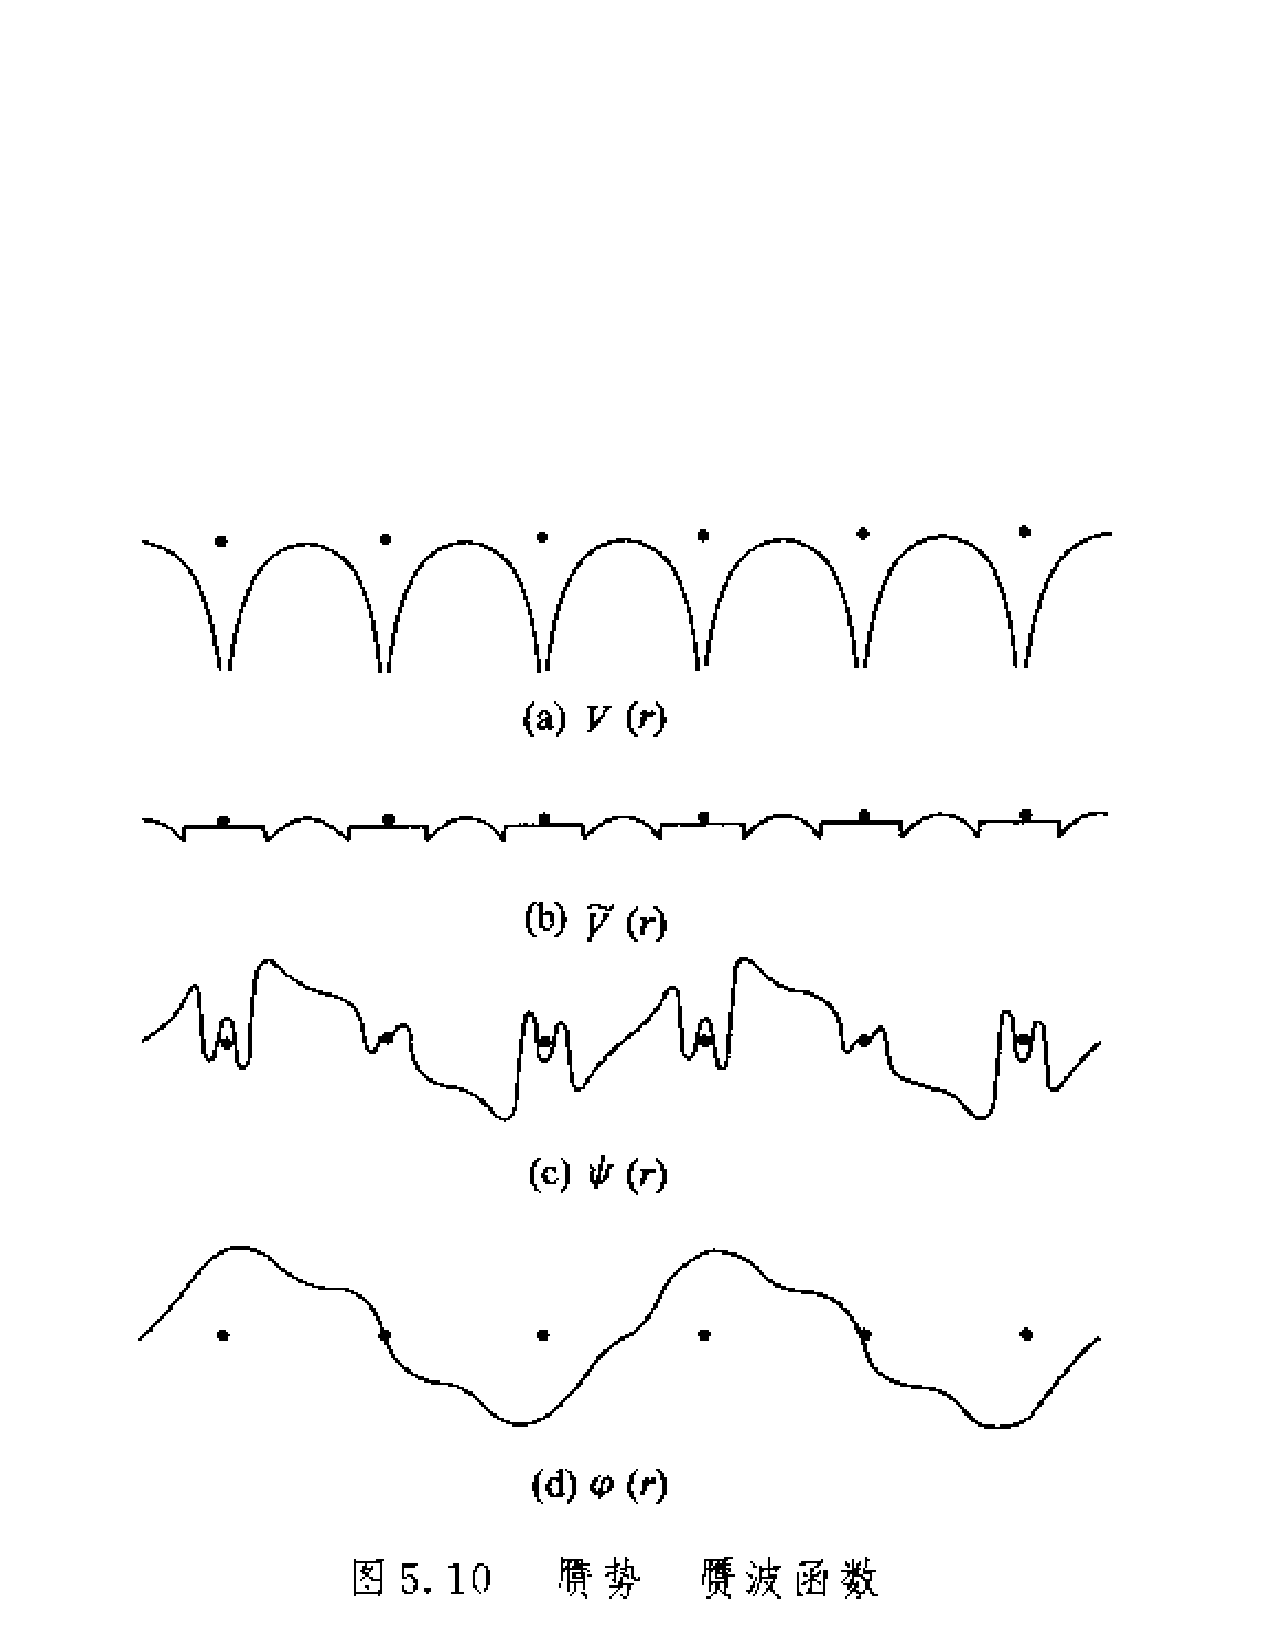
\includegraphics[height=0.8in,width=4.in,viewport=41 210 539 339,clip]{Figures/Pseudo_wave.pdf}
\caption{\tiny \textrm{The periodic Potential and the wave functions in crystal.}}%(与文献\cite{EPJB33-47_2003}图1对比)
\label{Potential-Wave}
\end{figure}
}

\frame
{
\frametitle{一维自由电子近似微扰}
\begin{figure}[h!]
\centering
%\hspace*{-10pt}
%\vspace*{-1.1in}
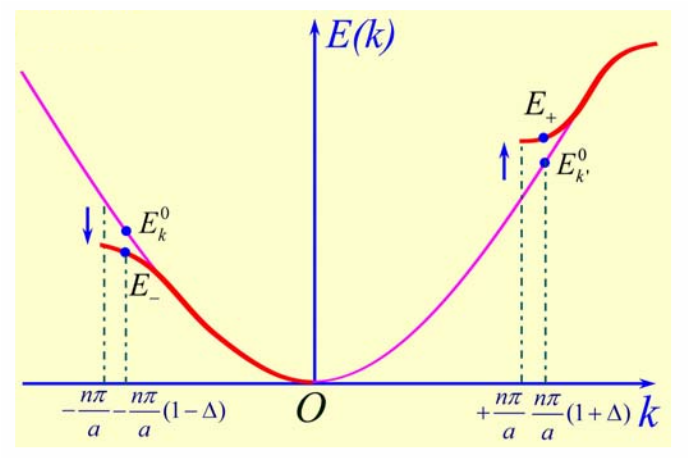
\includegraphics[height=1.5in,width=2.5in,viewport=5 5 700 450,clip]{Figures/Band_Gap-2.png}
%\caption{\tiny \textrm{The Band-structure from free-electron gas.}}%
\label{Band-Gap-2}
\end{figure} 
\begin{displaymath}
	\begin{aligned}
		&\hat H_0=-\dfrac{\hbar^2}{2m}\dfrac{\mathrm{d}^2}{\mathrm{d}x^2}+\={V} \longrightarrow \hat H=\hat H_0+\hat H^{\prime}=-\dfrac{\hbar^2}{2m}\dfrac{\mathrm{d}^2}{\mathrm{d}x^2}+\={V}+\underline{V(x)-\={V}}\\
		&\Psi_k^0(x)=\dfrac1{\sqrt V}\mathrm{e}^{\mathrm{i}k\cdot x} \longrightarrow \Psi_k(x)=\Psi_k^0(x)+\sum_{k^{\prime}\neq k}\dfrac{\langle k^{\prime}|\hat H^{\prime}|k\rangle}{E_k^0-E_{k^{\prime}}^0}\Psi_{k^{\prime}}^0(x)\\
		&\hat E_k^0=-\dfrac{\hbar^2k^2}{2m}+\={V} \longrightarrow E_k=%E_k^0+E^{\prime}=
		\dfrac{\hbar^2k^2}{2m}+\={V}+\sum_n{}^{\prime}\dfrac{|V_n|^2}{\frac{\hbar^2}{2m}[k^2-(k+2\pi\frac na)^2]}
	\end{aligned}
\end{displaymath}
}

\frame
{
\frametitle{一维自由电子简并微扰}
在波矢$k=\pm\frac{n\pi}{a}$位置,电子能量出现简并态,必须采用简并态微扰理论处理
\begin{figure}[h!]
\centering
%\hspace*{-10pt}
%\vspace*{-1.1in}
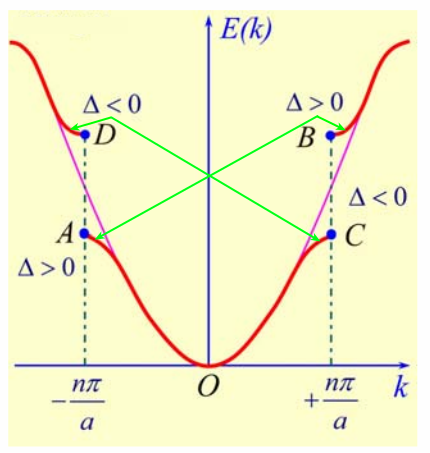
\includegraphics[height=1.3in,width=1.4in,viewport=0 5 420 450,clip]{Figures/Band_Gap-1.png}
%\caption{\tiny \textrm{The Band-structure from free-electron gas.}}%
\label{Band-Gap-1}
\end{figure} 
\begin{displaymath}
	E_{\textcolor{red}{\pm}}=\left\{
	\begin{aligned}
		&T_n+\={V}\textcolor{red}{+}\Delta^2T_n\bigg(\dfrac{2T_n}{|V_n|}\textcolor{red}{+}1\bigg)\\
		&T_n+\={V}\textcolor{red}{-}\Delta^2T_n\bigg(\dfrac{2T_n}{|V_n|}\textcolor{red}{-}1\bigg)
	\end{aligned}\right.
\end{displaymath}
这里$T_n=\frac{\hbar^2}{2m}\big(\frac{n\pi}a\big)^2$
}

\frame
{
\frametitle{自由电子气模型}
简并态微扰理论引起的能带裂分
\begin{figure}[h!]
\centering
%\hspace*{-10pt}
%\vspace*{-1.1in}
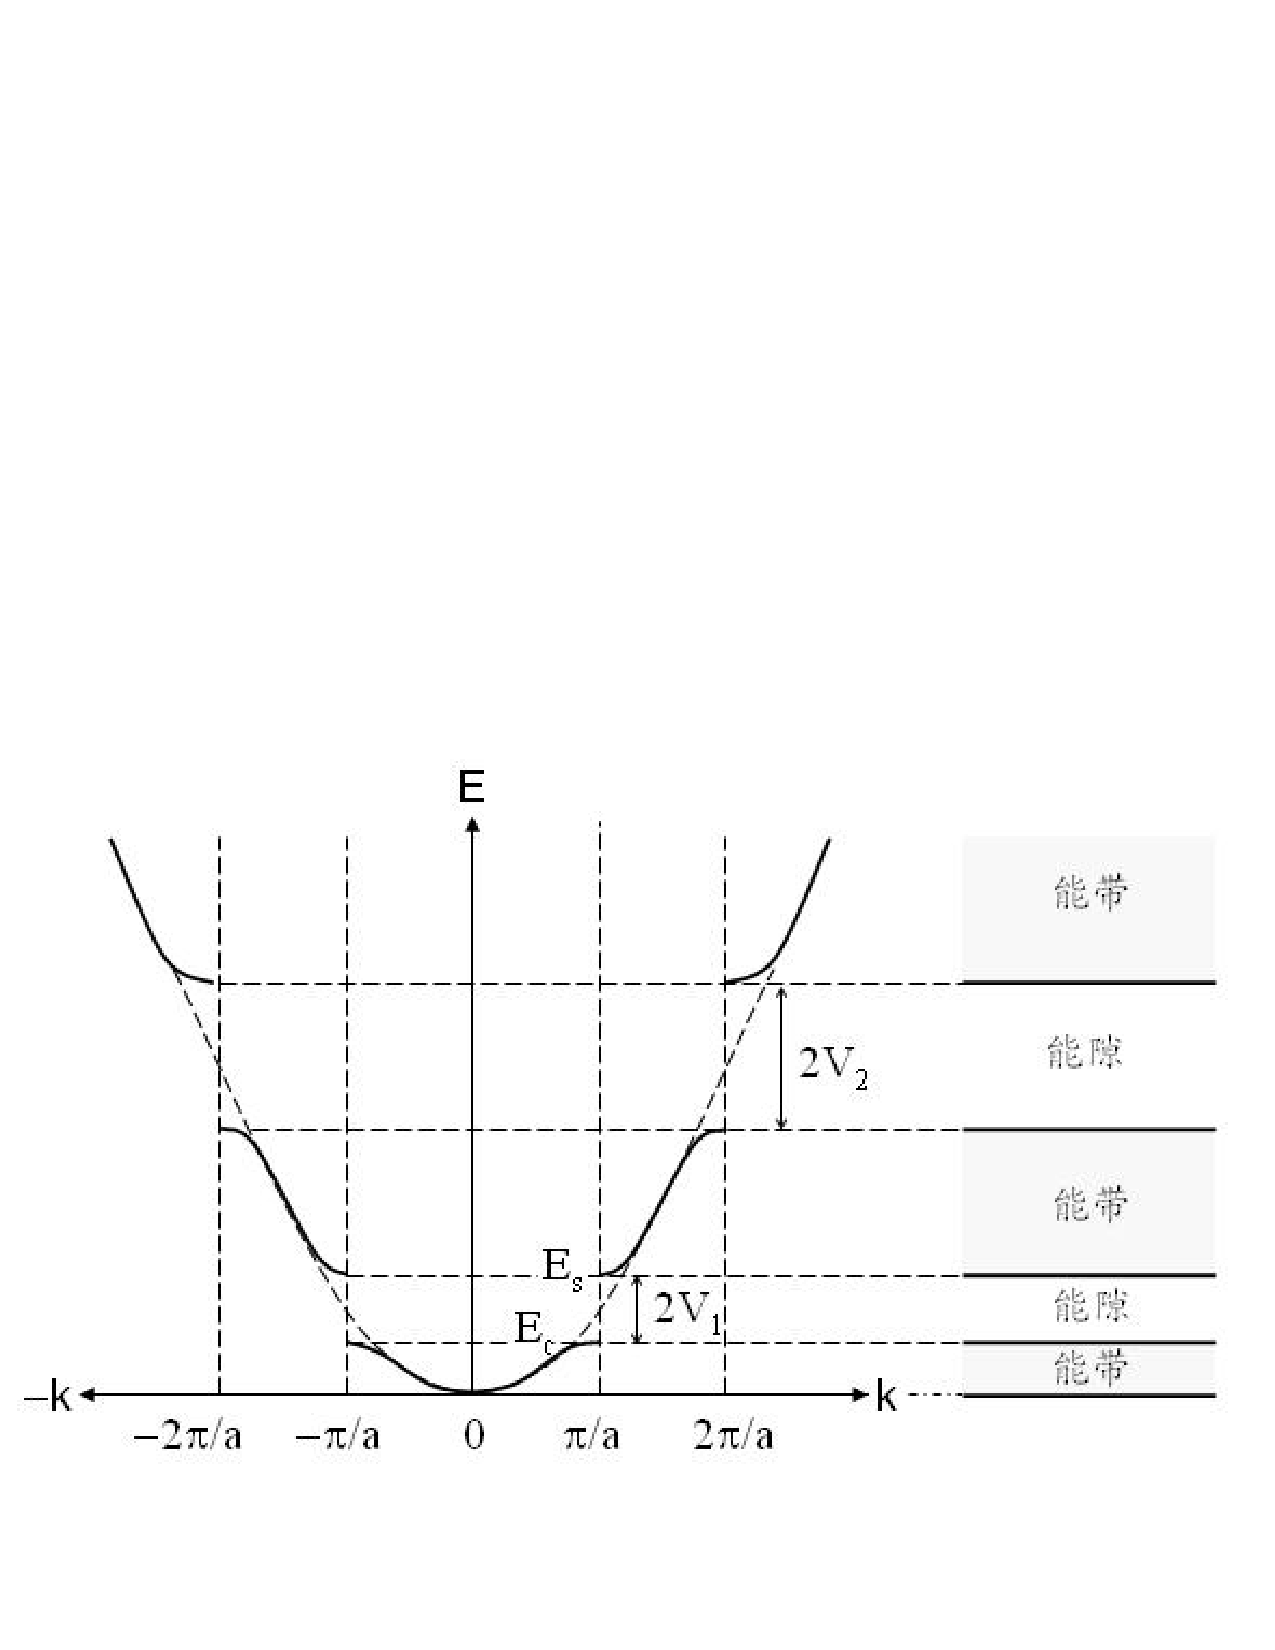
\includegraphics[height=2.1in,width=3.8in,viewport=10 90 570 380,clip]{Figures/Band_Gap.pdf}
\caption{\tiny \textrm{The Band-structure from free-electron gas.}}%
\label{Band-Gap-co}
\end{figure} 
}

\frame
{
\frametitle{紧束缚模型}
从分子轨道到能带
\begin{figure}[h!]
\centering
\hspace*{-0.29in}
\vspace*{-0.1in}
\subfigure[一维$\mathrm{H}$原子链]{
\label{fig:Hydrogen-1D}
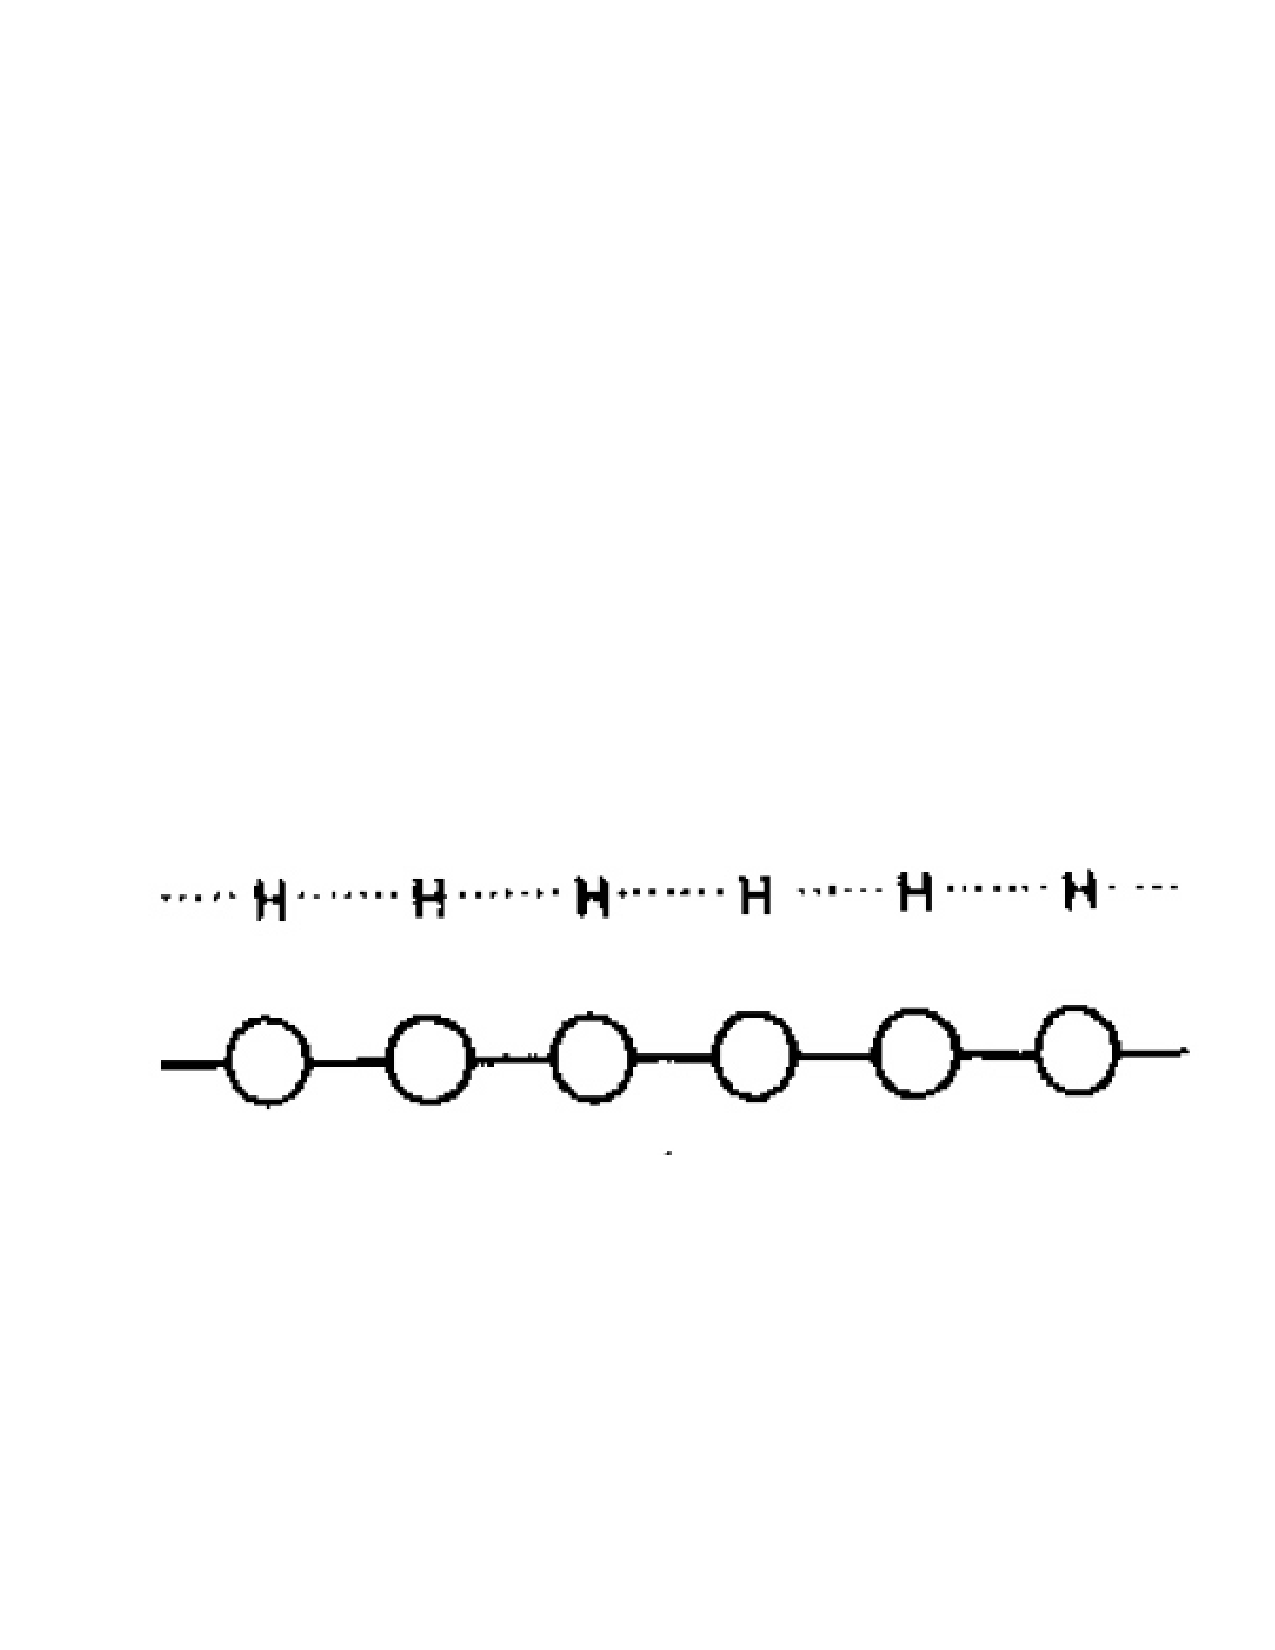
\includegraphics[height=0.25in,width=1.1in,viewport=70 255 570 375,clip]{Figures/Hydrogen-1D.pdf}}
\subfigure[$\mathrm{H}_n$分子轨道]{
\label{fig:Hydrogen-2-n}
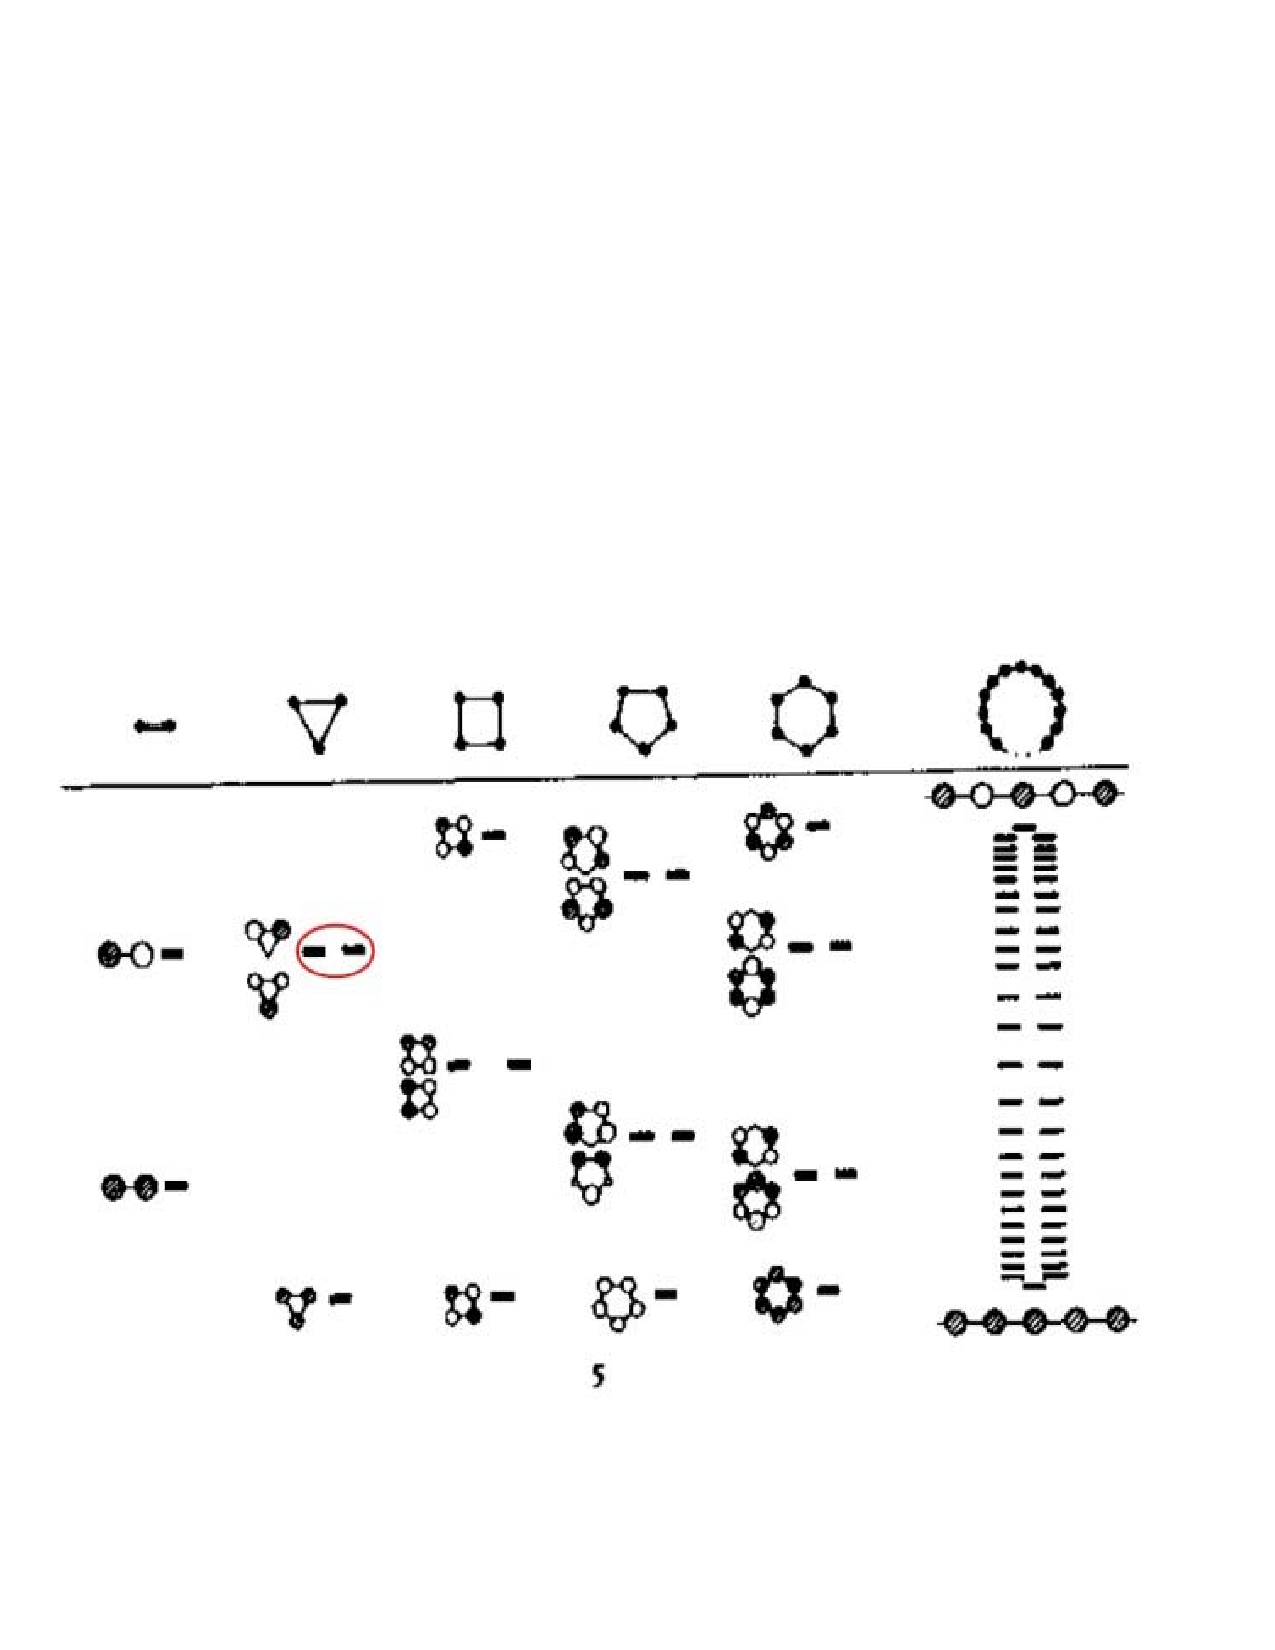
\includegraphics[height=0.8in,width=1.5in,viewport=30 140 545 480,clip]{Figures/Hydrogen-Mol-Orbital.pdf}}
\subfigure[分子波函数]{
\label{fig:Hydrogen-Psi}
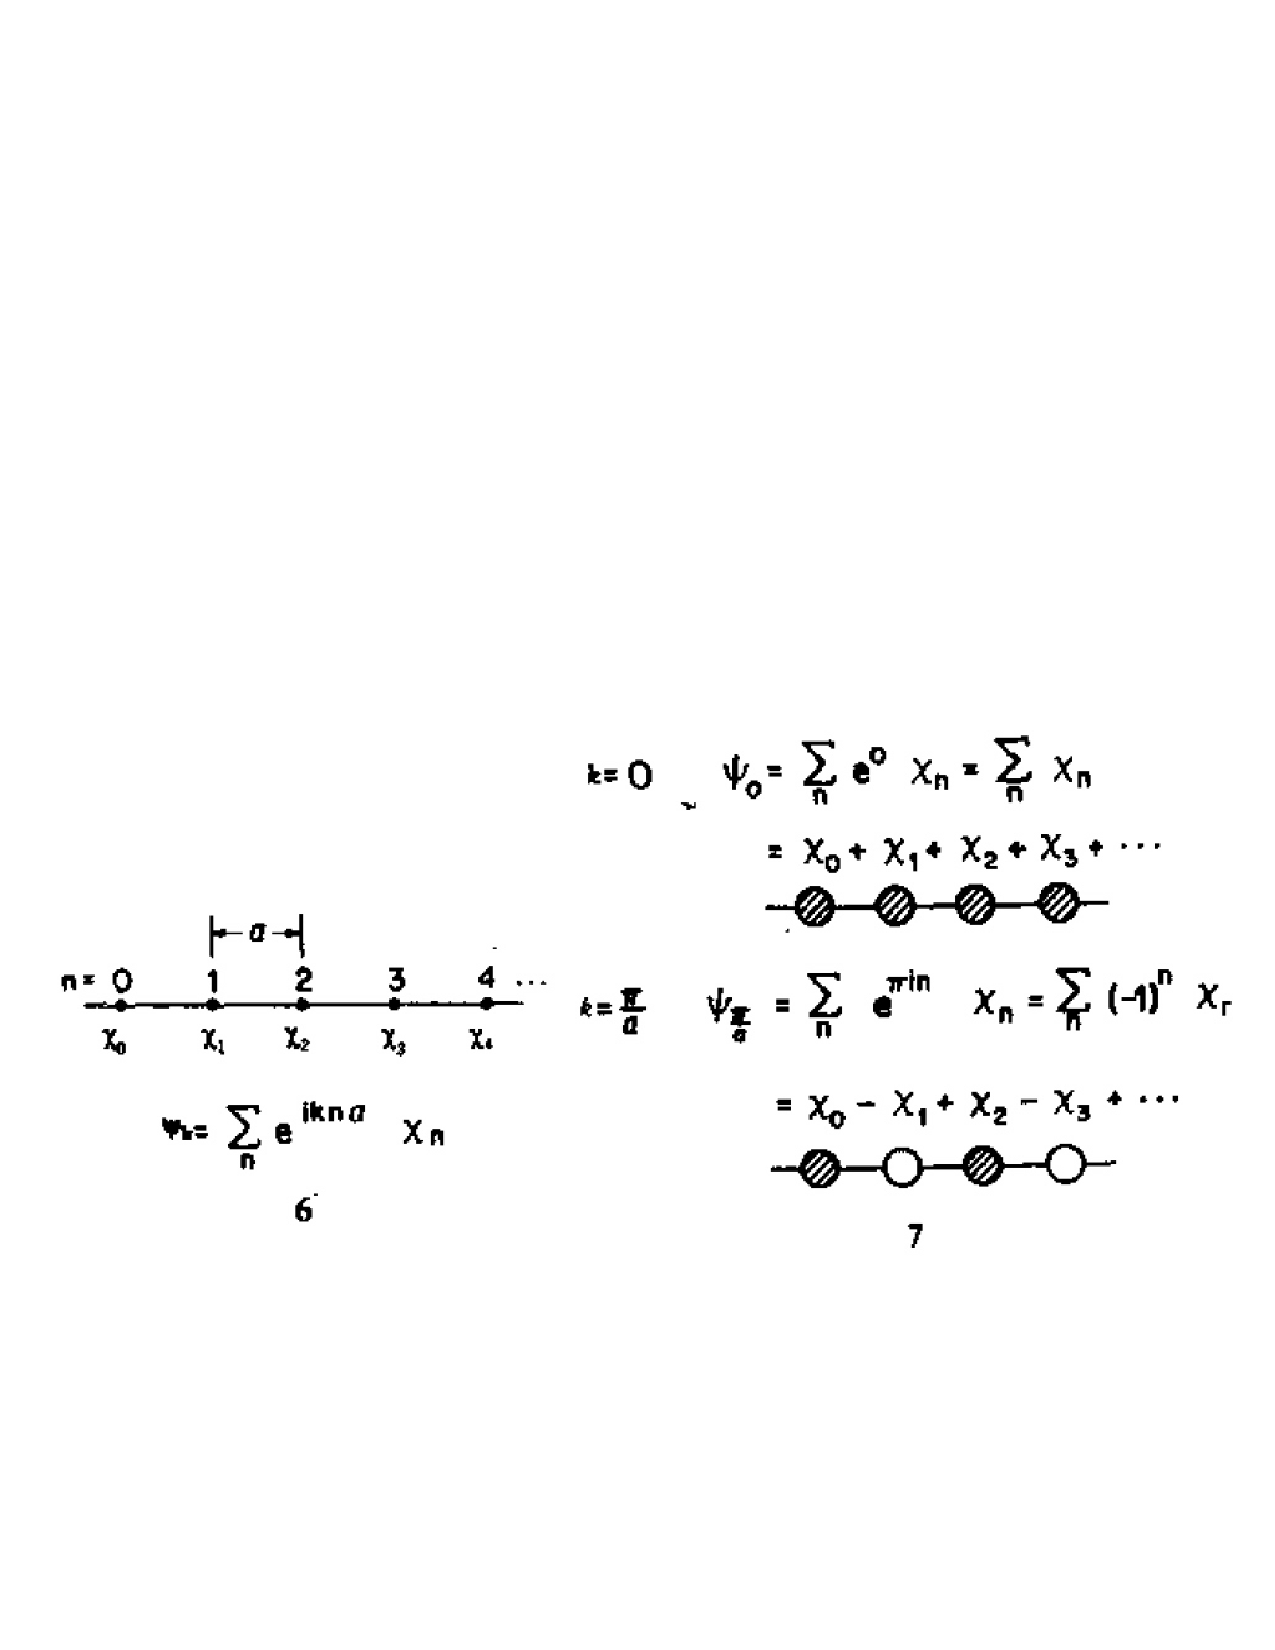
\includegraphics[height=0.5in,width=1.4in,viewport=25 218 595 440,clip]{Figures/Hydrogen-Psi.pdf}}\\
\vspace*{5pt}
\subfigure[分子轨道与能带]{
\label{fig:Hydrogen-Band-1D}
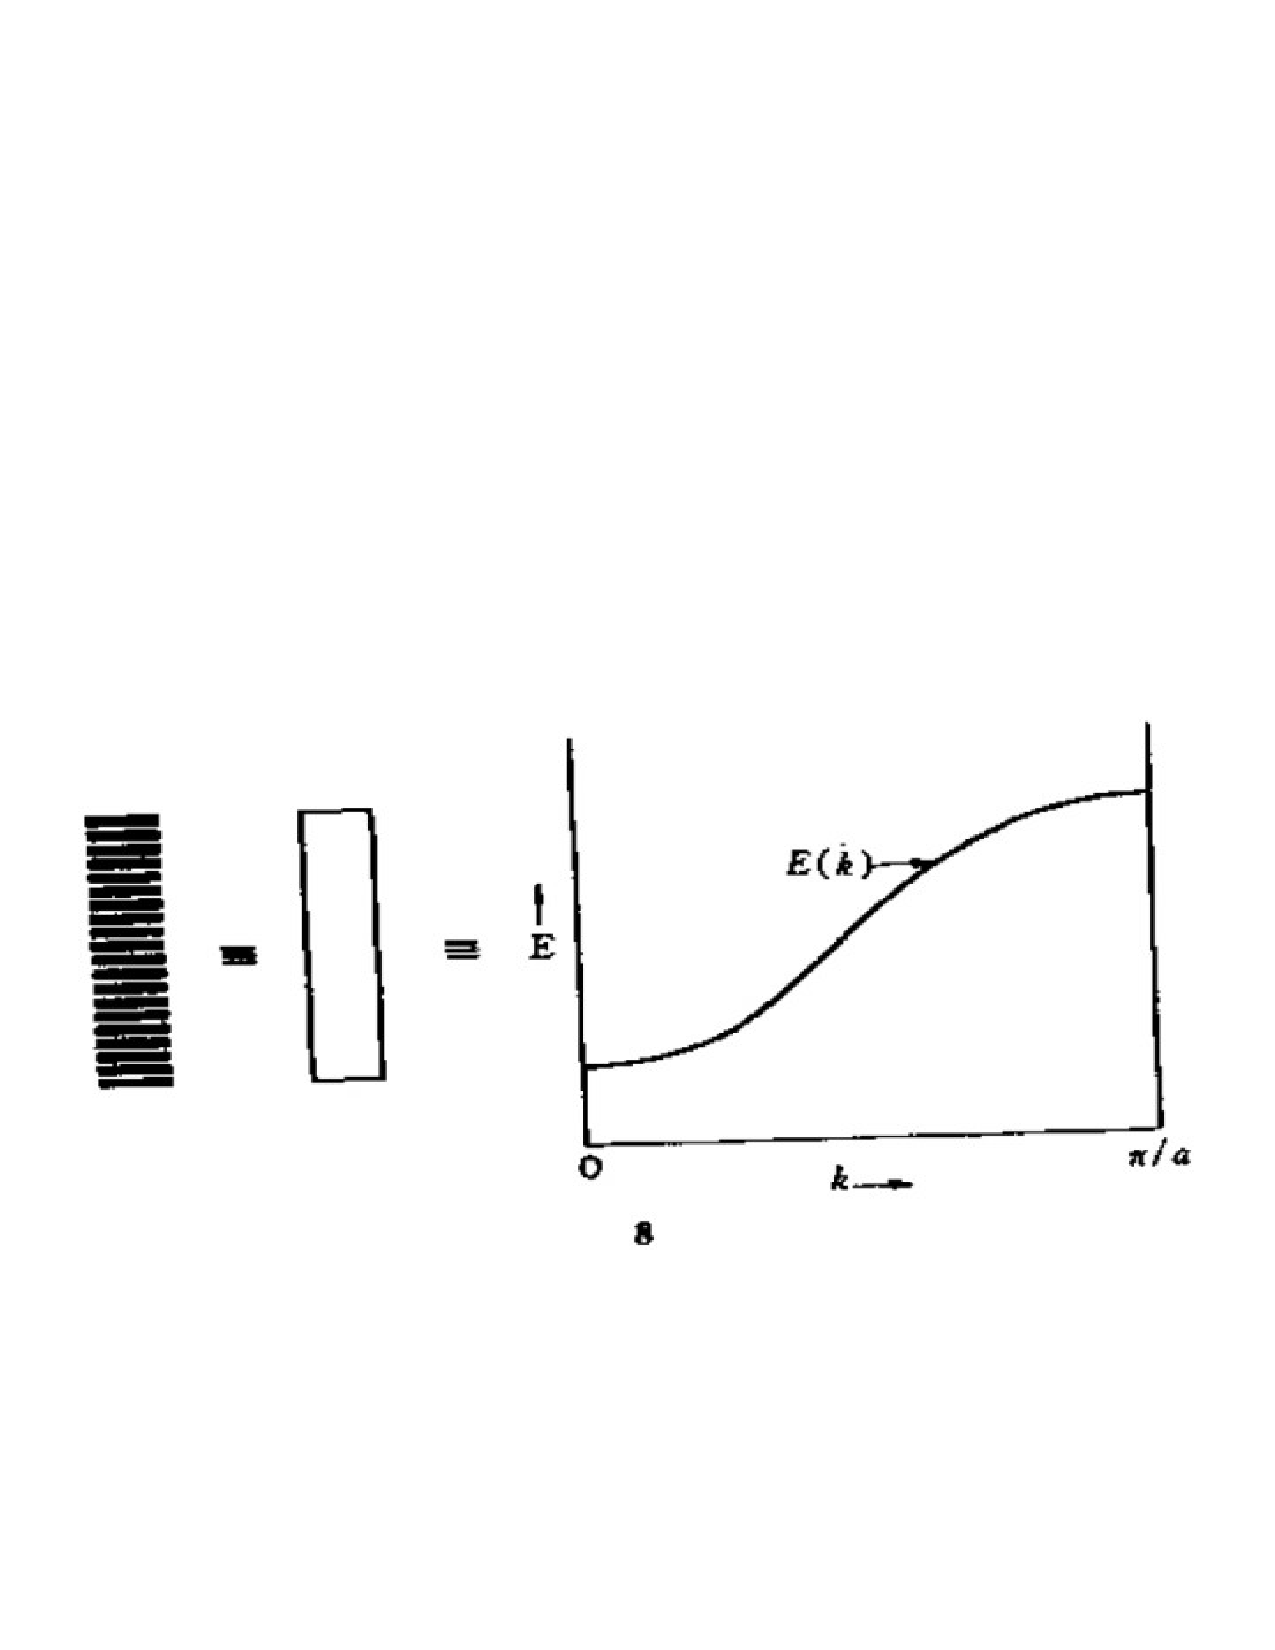
\includegraphics[height=0.6in,width=1.4in,viewport=35 215 575 450,clip]{Figures/Hydrogen-Band-1D.pdf}}
\subfigure[$d$\,轨道]{
\label{fig:Hydrogen-d-Band-1D}
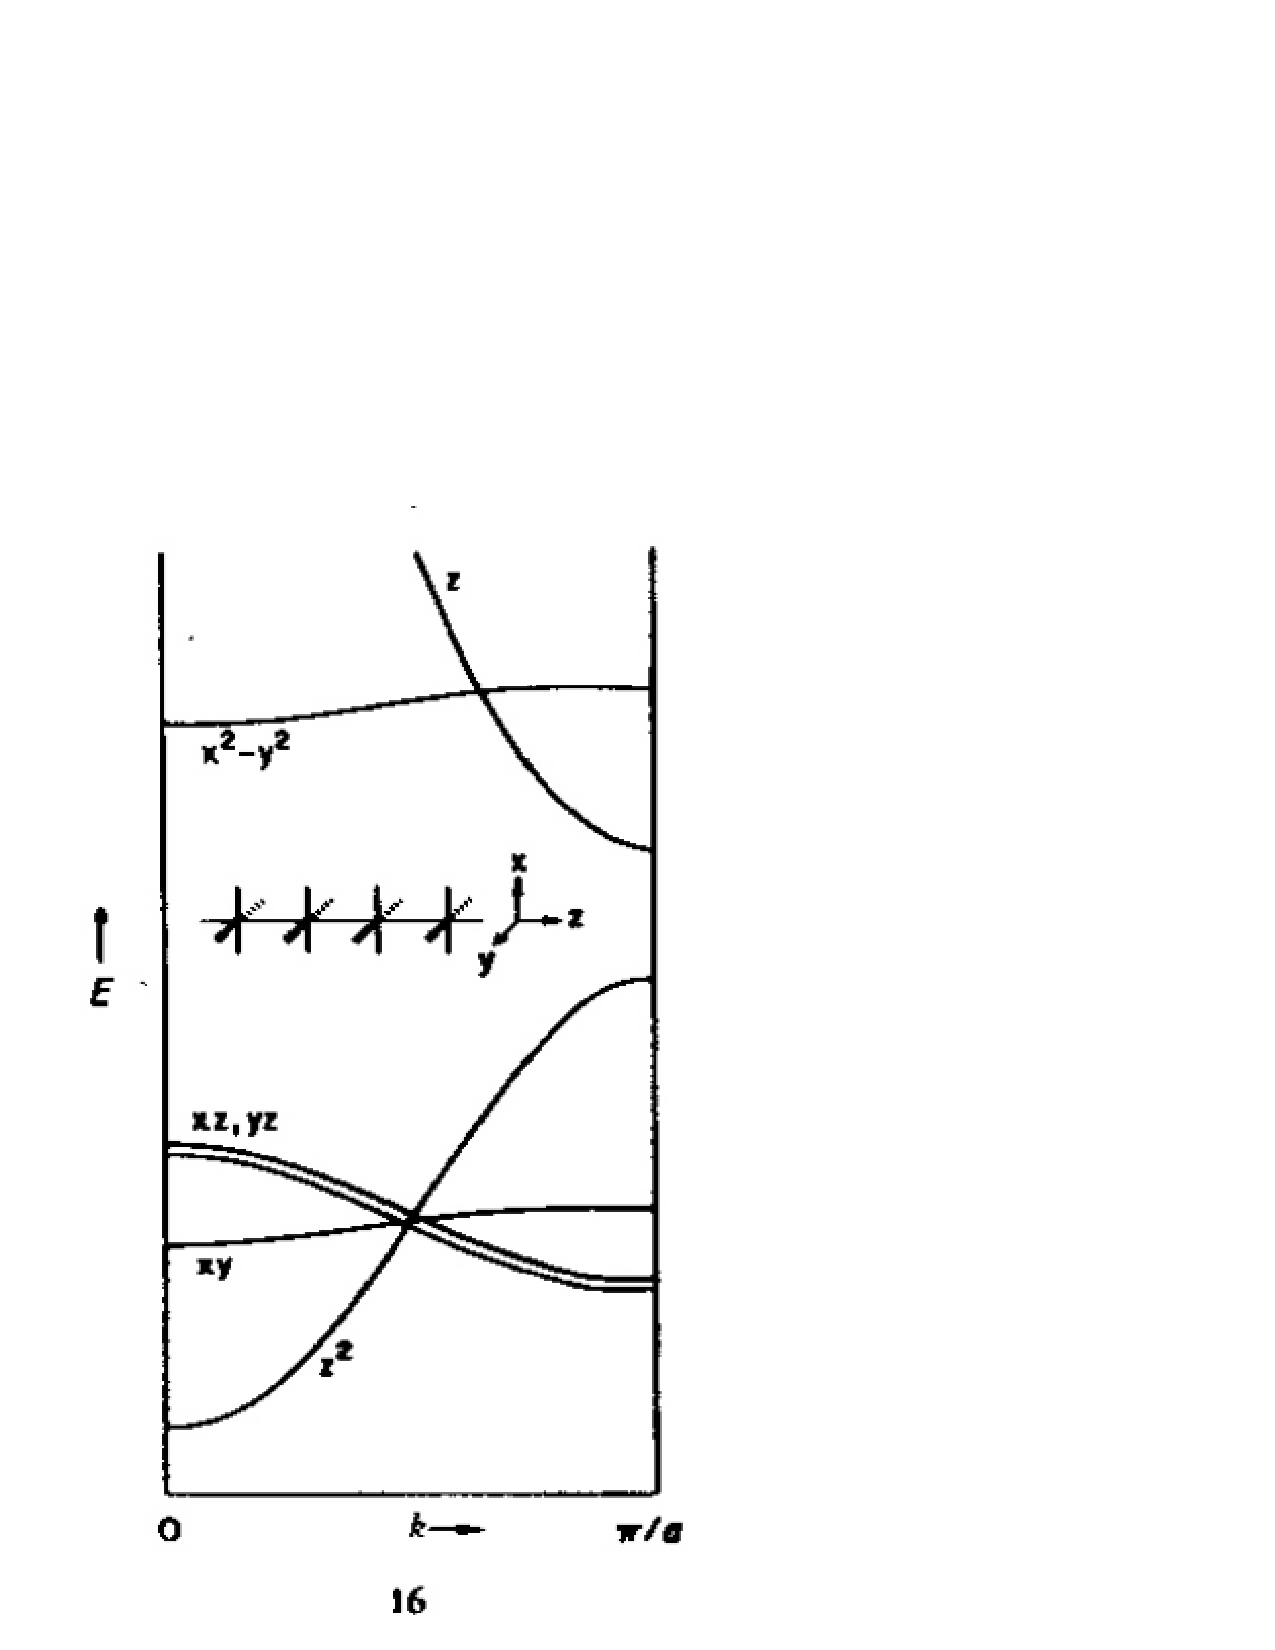
\includegraphics[height=1.0in,width=0.7in,viewport=40 45 330 535,clip]{Figures/Hydrogen-d-Band-1D.pdf}}
\caption{\tiny \textrm{The Band-structure from Molecular-orbital.}}%
\label{Band-Structure-local-orbit}
\end{figure} 
}

\subsection{能带、$\vec k$-空间与~\rm{Fermi~}面}
\frame
{
\frametitle{能带、$\vec k$空间与\textrm{Fermi}面}
\vspace{30pt}
\begin{figure}[h!]
\centering
\hspace*{-0.10in}
\subfigure[\textrm{Band structure}]{
\label{Band_Gap_Fermi-1}
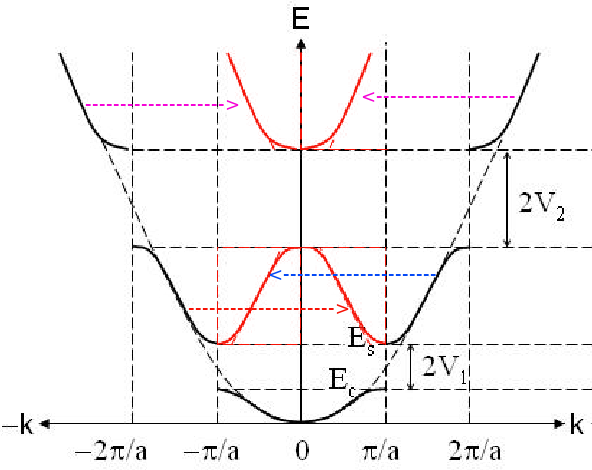
\includegraphics[height=1.6in,width=2.1in,viewport=0 0 480 350,clip]{Figures/Band_Brillouin_zone.png}}
\subfigure[\textrm{Brillouin Zone}]{
\label{Band_Gap_Fermi-2}
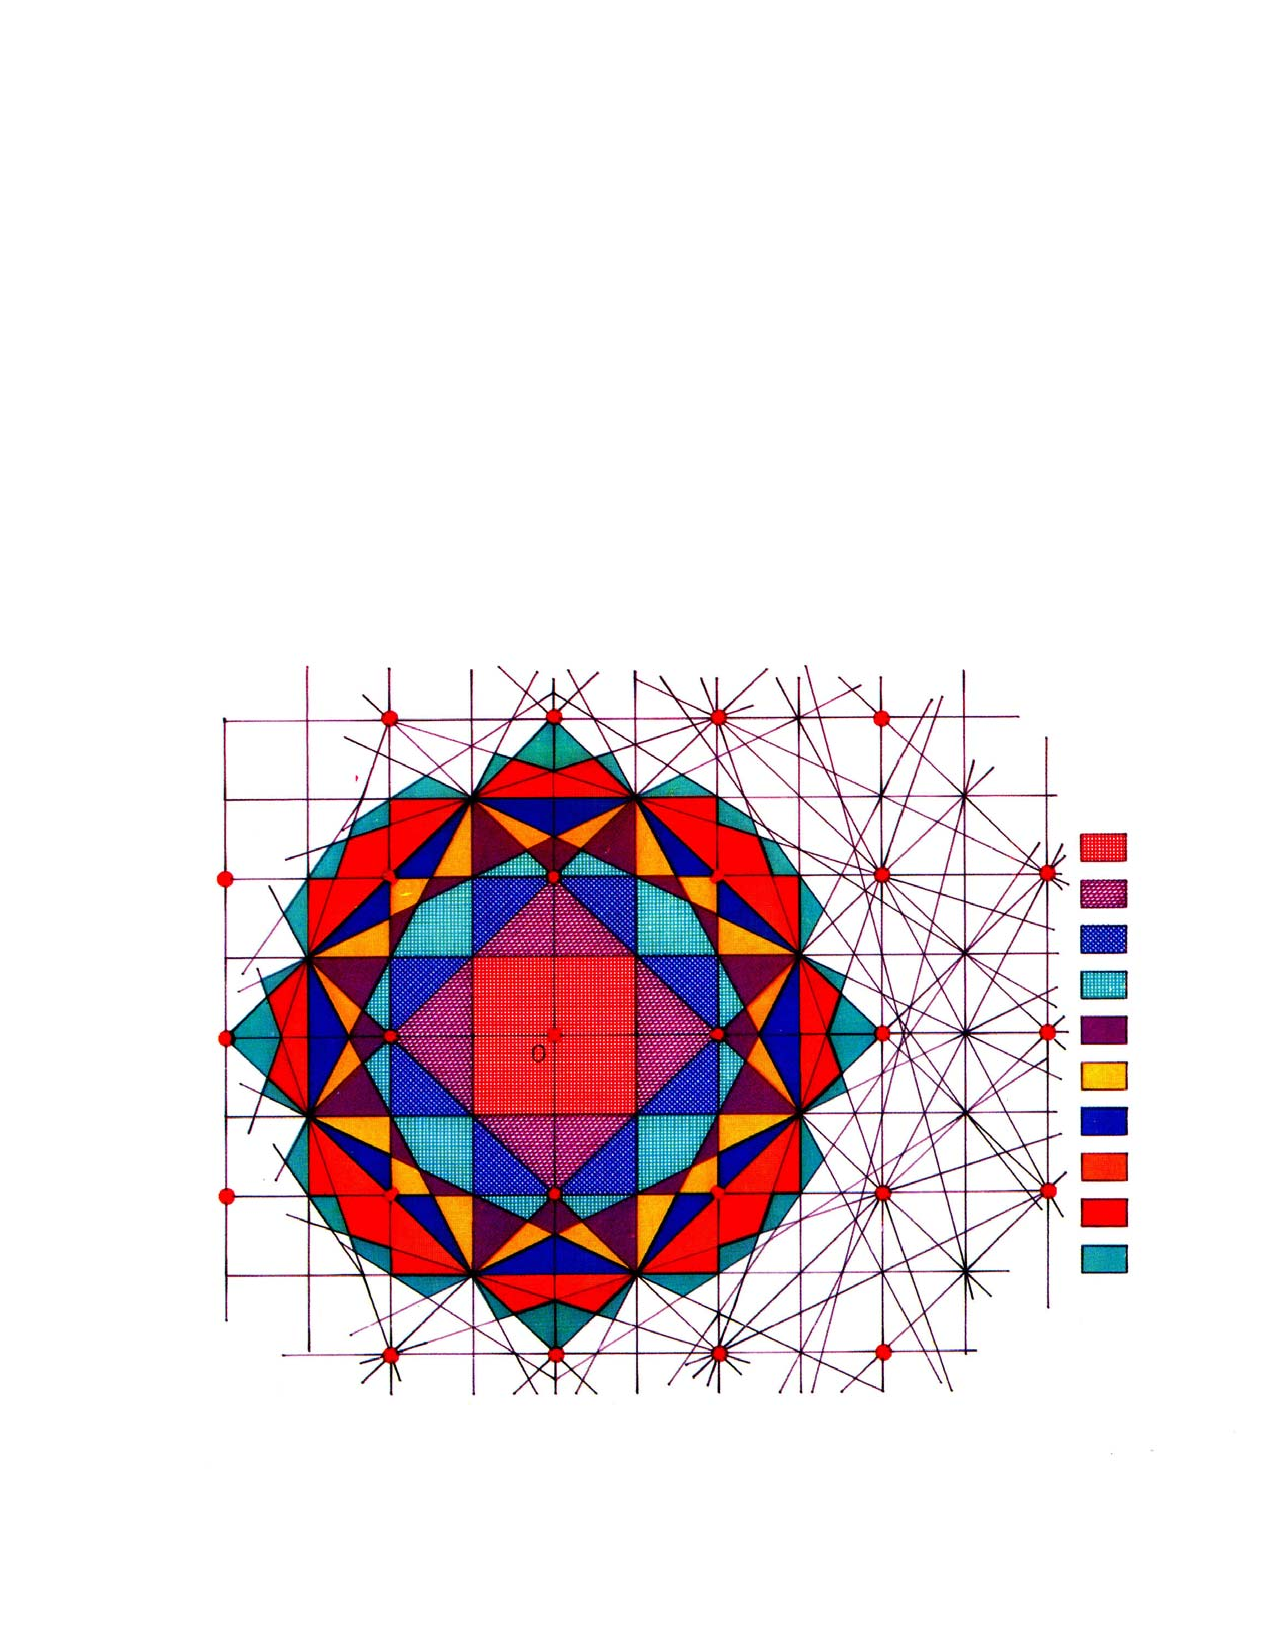
\includegraphics[height=1.28in,width=1.75in,viewport=100 120 545 470,clip]{Figures/2D_Brillouin-Zone.pdf}}
\label{Band_Gap_Fermi}
\end{figure}
}

\frame
{
	\frametitle{简单立方体系的\textrm{Brillouin}区与能带}
\vspace{10pt}
\begin{figure}[h!]
\centering
\hspace*{-0.28in}
\subfigure[\textrm{Brillouin Zone of Cubic lattice}]{
\label{Brillouin_Zone_Cubic-1}
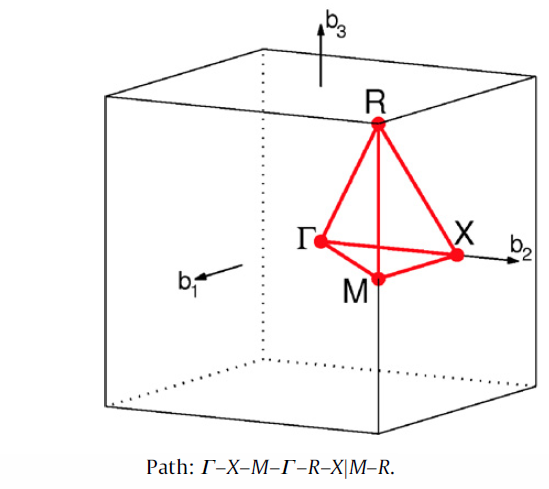
\includegraphics[height=2.1in,width=2.0in,viewport=90 0 550 500,clip]{Figures/Brillouin-Zone_CUB.png}}
\subfigure[\textrm{Band Structure of \ch{SrSnO3}}]{
\label{Band_Gap_SrSnO3-1}
\vspace*{-1.00in}
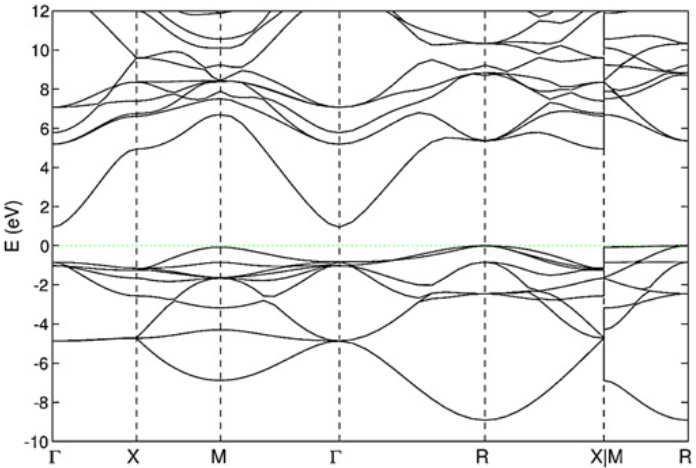
\includegraphics[height=2.10in,width=1.75in,viewport=0 0 710 550,clip]{Figures/Band-Struct_SrSnO3.png}}
\label{Band_Gap_CUB_SrSnO3}
\end{figure}
}

\frame
{
	\frametitle{面心立方体系的\textrm{Brillouin}区与能带}
\vspace{10pt}
\begin{figure}[h!]
\centering
\hspace*{-0.30in}
\subfigure[\textrm{Brillouin Zone of FCC lattice}]{
\label{Brillouin_Zone_FCC}
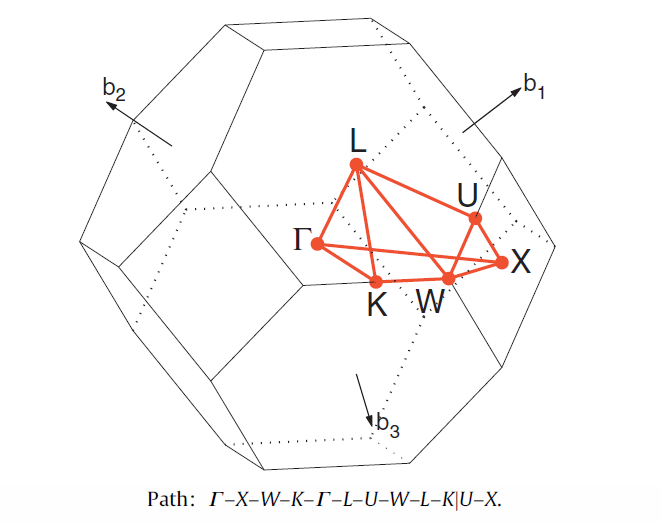
\includegraphics[height=1.9in,width=1.8in,viewport=75 0 560 520,clip]{Figures/Brillouin-Zone_FCC.png}}
\subfigure[\textrm{Band structure of \ch{CdS}}]{
\label{Band_Gap_CdS}
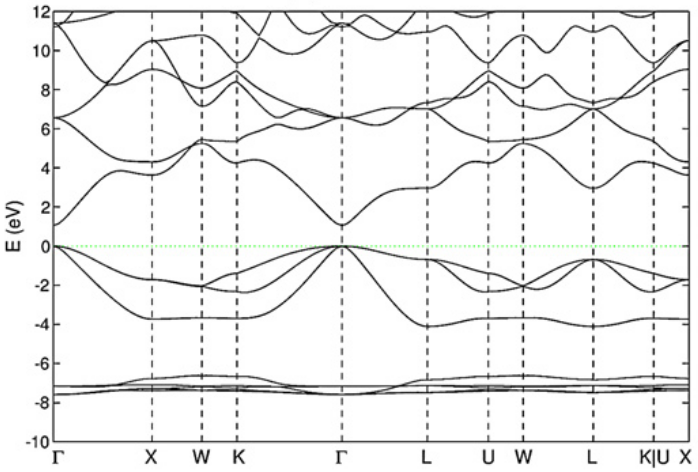
\includegraphics[height=2.10in,width=1.95in,viewport=0 0 700 520,clip]{Figures/Band-Struct_CdS.png}}
\label{Band_Gap_FCC_CdS}
\end{figure}
}

\frame
{
	\frametitle{体心立方体系的\textrm{Brillouin}区与能带}
\vspace{10pt}
\begin{figure}[h!]
\centering
\hspace*{-0.30in}
\subfigure[\textrm{Brillouin Zone of BCC lattice}]{
\label{Brillouin_Zone_BCC}
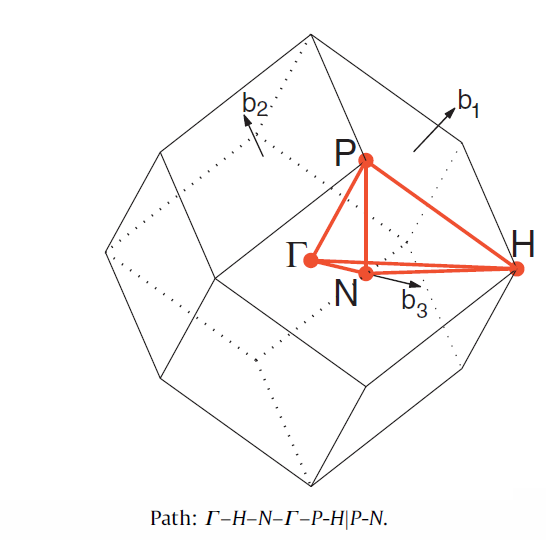
\includegraphics[height=2.1in,width=1.9in,viewport=80 0 550 520,clip]{Figures/Brillouin-Zone_BCC.png}}
\subfigure[\textrm{Band structure of \ch{GeF4}}]{
\label{Band_Gap_GeF4}
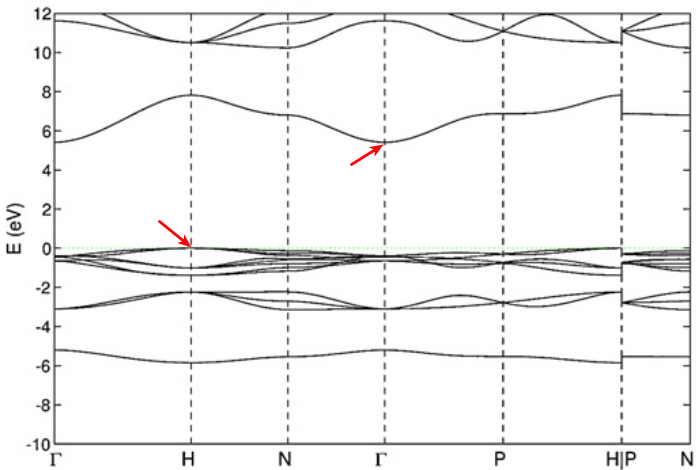
\includegraphics[height=2.10in,width=1.95in,viewport=0 0 700 500,clip]{Figures/Band-Struct_GeF4.png}}
\label{Band_Gap_BCC_GeF4}
\end{figure}
}

\subsection{固体能带计算方法}
\frame
{
%\frametitle{The methods on band structure calculation}
\frametitle{固体能带计算方法}
%\vskip 10pt
%\textrm{The mainly difference of all these methods below: the basis sets and the construction of the potential}
\vskip 10pt
常用的计算方法
\begin{itemize}%[+-| alert@+>]
%\begin{enumerate}%[+-| alert@+>]
\setlength{\itemsep}{12pt}
%  \item \textrm{Plane wave and the pseudo-potential}
	\item	平面波方法
	\item	正交平面波\textrm{(The orthogonalized plane wave, OPW)}和赝势\textrm{(Pseudo-potential, PP)}方法\upcite{Singh,PRB41-7892_1990,JPCM6-8245_1994}
	\item	缀加平面波\textrm{(Augmented plane wave, APW)}方法
	\item	\textrm{MT}轨道\textrm{(Muffin-tin orbitals, MTO)}方法
	\item	投影子缀加波\textrm{(Projector Augmented Wave, PAW)}方法\upcite{PRB50-17953_1994,PRB59-1758_1999}
\end{itemize}
\vskip 5pt 各种方法的\textcolor{red}{主要区别}:~\textcolor{blue}{势函数的处理}与\textcolor{blue}{所选基函数类型}不同
}

\frame
{
	\frametitle{球形势对平面波的散射}
\begin{figure}[h!]
\centering
\vspace*{-0.26in}
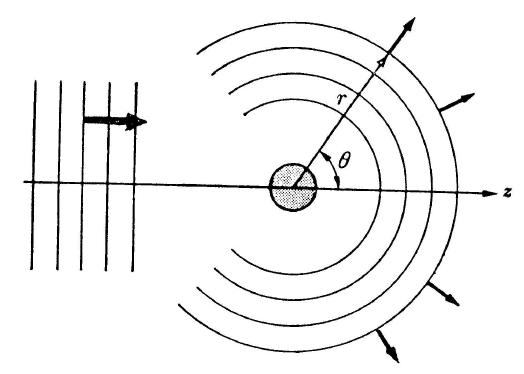
\includegraphics[height=1.90in,width=2.48in,viewport=0 0 400 300,clip]{Figures/Pseudo-scatter.jpg}
\caption{\fontsize{5.5pt}{4.2pt}\selectfont{\textrm{Schematic illustration of scattering of a plane wave by a spherical potential.}}}%(与文献\cite{EPJB33-47_2003}图1对比)
\label{Pseudo-scatter}
\end{figure}
\vspace*{-0.1in}
\fontsize{7.5pt}{6.2pt}\selectfont{
入射平面波
$$\mathrm{e}^{\mathrm{i}\vec q\cdot\vec r}=4\pi\sum_{lm}\mathrm{i}^lj_l(\vec q\cdot\vec r)Y_{lm}^{\ast}(\hat{\vec q})Y_{lm}(\hat{\vec r})=\sum_{l}(2l+1)\mathrm{i}^lj_l(qr)P_{l}(\cos\theta)$$
%$$\mathrm{e}^{\mathrm{i}\vec q\cdot\vec r}=\mathrm{e}^{\mathrm{i}qr\cos(\theta)}=\sum_{l}(2l+1)\mathrm{i}^lj_l(qr)P_{l}[\cos(\theta)]$$
}
}

\frame
{
	\frametitle{势阱与相移}
\begin{figure}[h!]
\centering
\vspace*{-0.26in}
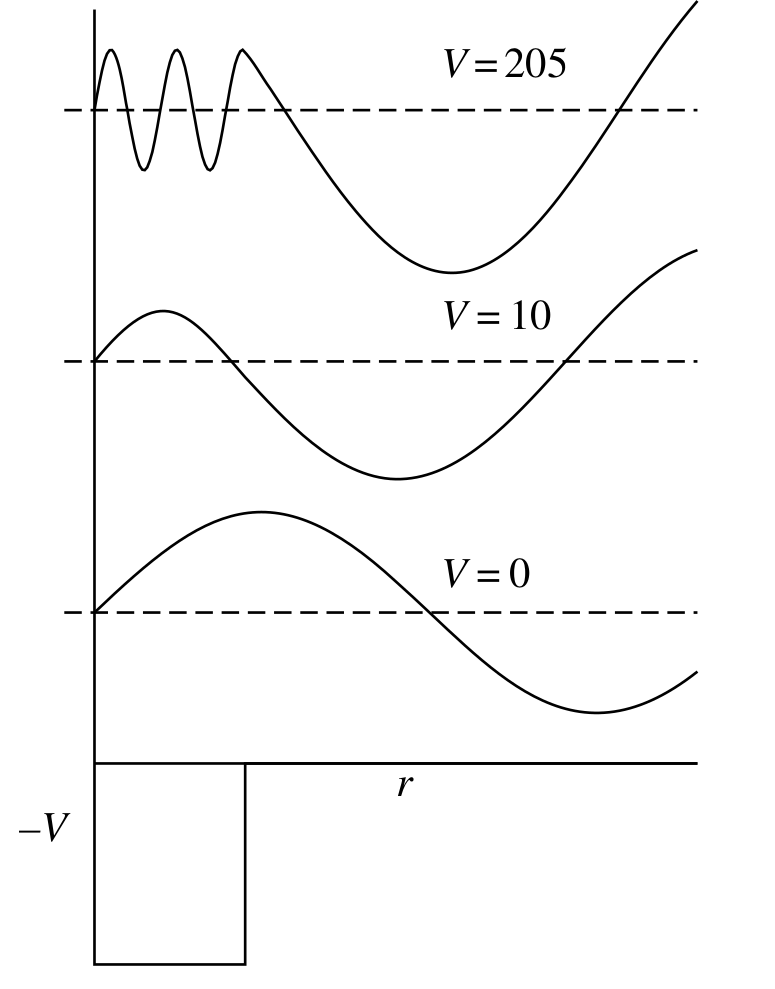
\includegraphics[height=1.85in,width=1.3in,viewport=0 0 750 1050,clip]{Figures/Radial_wave_functions_for_various_square_well_potential.png}
\caption{\fontsize{5.5pt}{4.2pt}\selectfont{\textrm{The radial wave functions for \textit{l}=0 for various square well potential depths.}}}%(与文献\cite{EPJB33-47_2003}图1对比)
\label{Pseudo-scatter}
\end{figure}
\vspace*{-0.1in}
\fontsize{7.5pt}{6.2pt}\selectfont{
平面波经散射后出射,波函数变为
$$\Psi_l^{>}(\varepsilon,r)=C_l\bigg[j_l(\kappa r)-\tan\eta_l(\varepsilon)n_l(\kappa r)\bigg]\quad\text{其中}\kappa^2=\varepsilon$$
根据散射理论,能量为$\varepsilon$的电子经单个势阱散射偏转$\theta$后,波函数的振幅可以表示为
	\begin{displaymath}
		t(\theta)=\dfrac{4\pi}{\kappa}\sum_l(2l+1)[\mathrm{exp}(2\mathrm{i}\eta_l(\varepsilon))-1]P_l(\cos\theta)
	\end{displaymath}
%$$t(\theta)=\dfrac{4\pi}{\sqrt\varepsilon}\sum_l(2l+1)\bigg[\mathrm{e}^{2\mathrm{i}\eta_l(\varepsilon)}-1\bigg]P_l(\cos\theta)$$
%$$\eta_l(\varepsilon)=p_l\pi+\delta_l(\varepsilon)$$
}
}

\frame
{
	\frametitle{球形势散射的相移与赝势}
\begin{figure}[h!]
\centering
\vspace*{-0.20in}
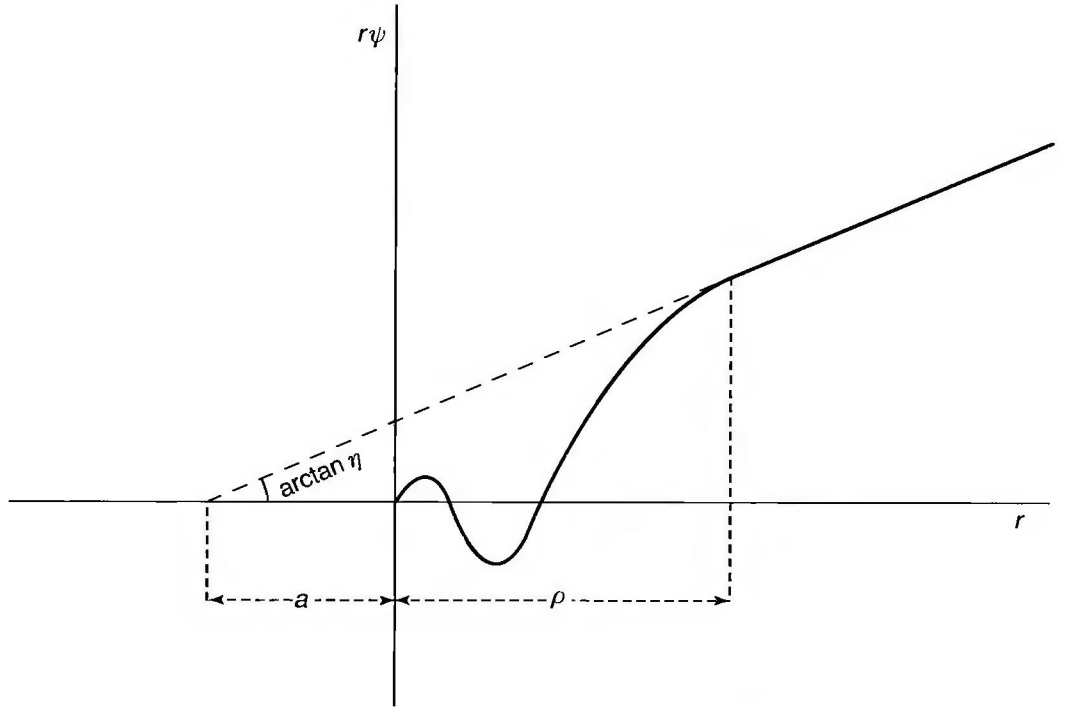
\includegraphics[height=1.20in,width=1.77in,viewport=0 0 1150 750,clip]{Figures/Pseudo-scatter-2.png}
\caption{\fontsize{4.5pt}{3.2pt}\selectfont{\textrm{Radial wave-function $\phi=r\psi$ for low-energy scattering as illustrated in a figure from the 1934 and 1935 papers of Fermi and coworkers for low-energy electron scattering from atoms and neutron scattering from nuclei. The node in the wave-function near the origin show that the potential is attractive and strong enough to have bound states. The cross-section for scattering from the localized potential is determined by the phase shift and is the same for weaker pseudo-potential with the same phase shift modulo $2\pi$.}}}%(与文献\cite{EPJB33-47_2003}图1对比)
\label{Pseudo-scatter-2}
\end{figure}
\fontsize{7.5pt}{6.2pt}\selectfont{
对于球形势散射,相移可由径向波函数计算
$$\tan\eta_l(\varepsilon)=\dfrac{R\frac{\mathrm{d}}{\mathrm{d}r}j_l(\kappa r)|_R-D_l(\varepsilon)j_l(\kappa R)}{R\frac{\mathrm{d}}{\mathrm{d}r}n_l(\kappa r)|_R-D_l(\varepsilon)n_l(\kappa R)}$$
$$\mbox{其中~}D_l(\varepsilon,r)\equiv r\psi_l^{\prime}(r)/\psi_l(r)=r\dfrac{\mathrm{d}}{\mathrm{d}r}\ln\psi_l(r)$$
同时相移与波函数节点的关系为:$$\eta_l(\varepsilon)=p_l\pi+\delta(\varepsilon)$$}
}

%\frame
%{
%\begin{figure}[h!]
%\centering
%\vskip -3pt
%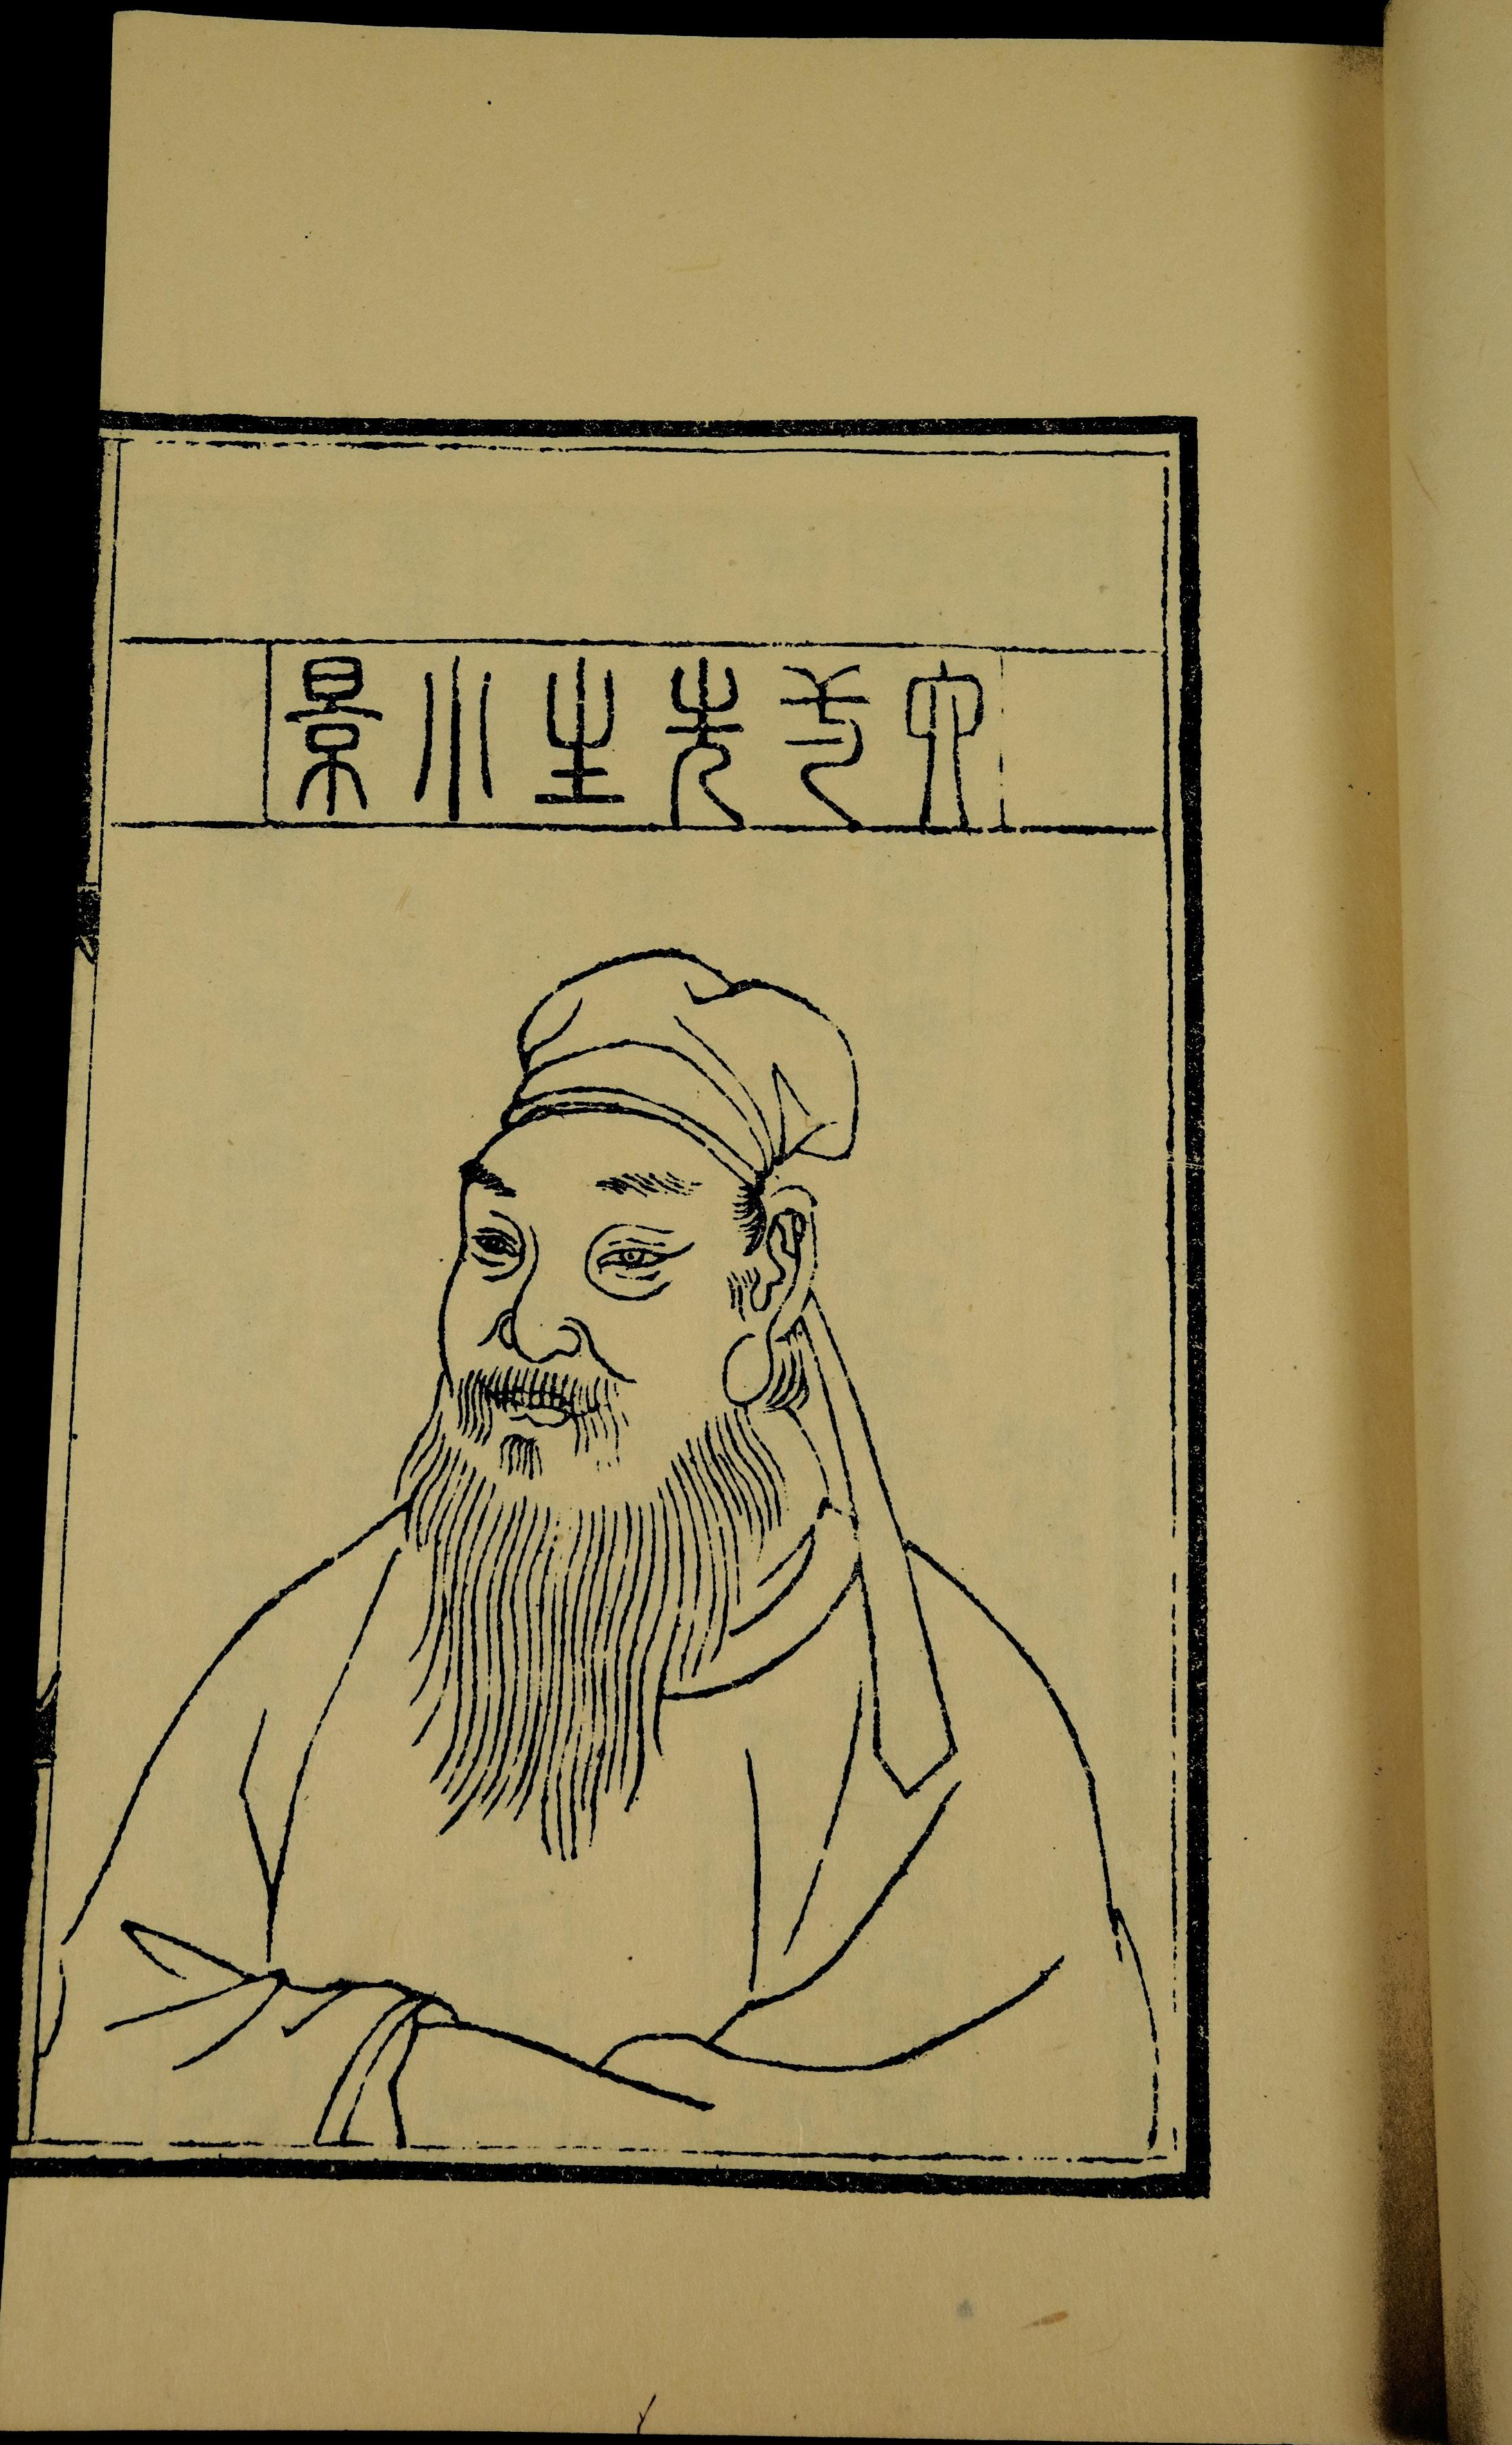
\includegraphics[height=2.5in,width=1.7in,viewport=0 0 600 850,clip]{Figures/Ouyang_Xiu-2.jpg}
%\hskip 20pt
%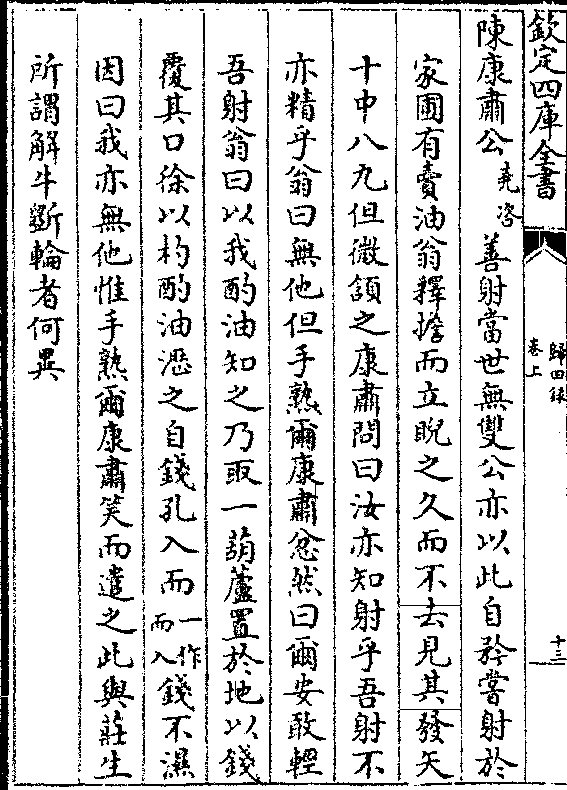
\includegraphics[height=2.5in,width=1.7in,viewport=0 0 600 790,clip]{Figures/Sale_Oil_Ouyang.png}
%\label{Sale_Oil_Ouyang}
%\caption{\tiny \textrm{欧阳修的《归田录\!$\cdot$\!卖油翁》.}}%(与文献\cite{EPJB33-47_2003}图1对比)
%\end{figure}
%}
%
\frame
{
	\frametitle{\textit{ab~initio}和\textrm{first~principle}}
	\begin{itemize}
		\item \textit{ab~initio}是拉丁文词汇(\textrm{Latin~term}),其含义是\textrm{``from the beginning''},由拉丁文\textit{ab}~\textrm{(``from'')}+\textit{initio}\textrm{(``beginning'')}合成,后者是\textit{initium}的单数夺格\footnote{夺格\textrm{(ablative)},又称离格或从格,语法功能上表示某些词汇的状语。拉丁文\textit{initium}的意思是"开始、初始"。}
		\item \textit{ab~initio}常用于法律和科学领域,如从头计算法(\textit{ab~initio}~\textrm{method})。法律中,\textit{ab~initio}表示"一开始即如此,而非法院宣判之后"。
		\item \textrm{first~principle}指从基本的物理学定律出发,不外加假设与经验拟合的推导与计算。
		\item 在物理学领域,\textrm{first~principle}(第一性原理)和\textit{ab~initio}(从头计算)含义上是等价的。例如利用\textrm{Schr\"odinger}方程在一些近似条件下求解电子结构,但无须依赖实验数据得到拟合参数的方法,就是第一原理或从头计算法。
	\end{itemize}
}

\frame
{
%	\frametitle{\textrm{DFT-SCF}}
\begin{figure}[h!]
\vspace*{-0.25in}
\centering
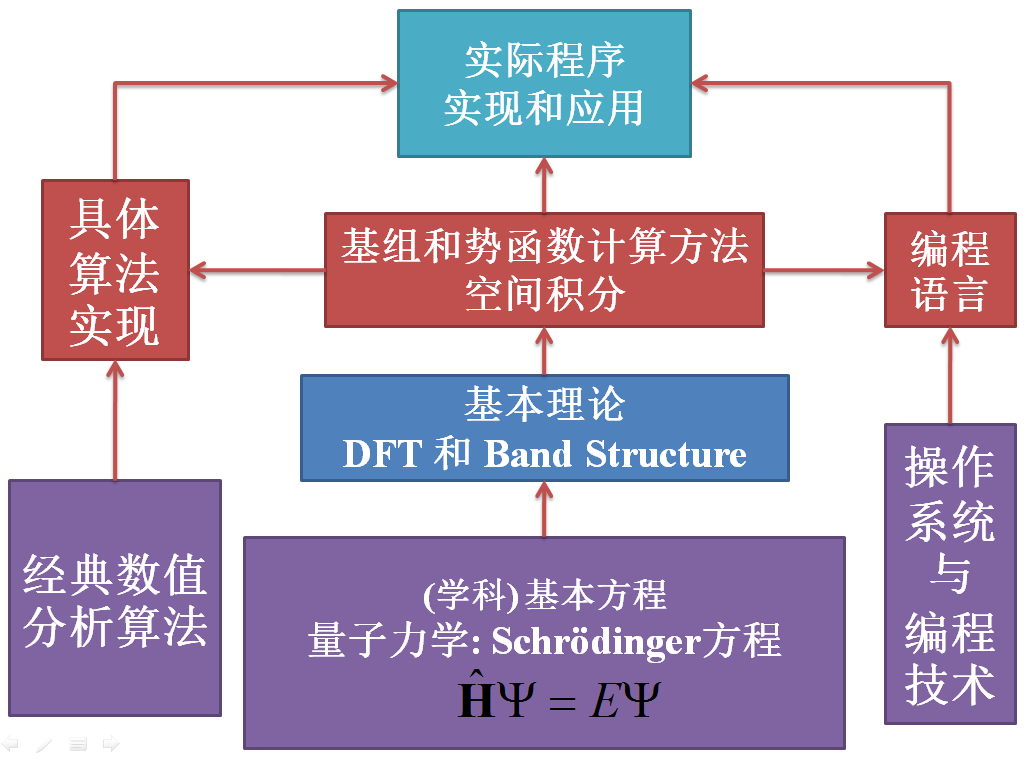
\includegraphics[height=2.80in,width=4.95in,viewport=5 3 1250 780,clip]{Figures/Method_Procedure.png}
%\caption{\tiny \textrm{Pseudopotential for metallic sodium, based on the empty core model and screened by the Thomas-Fermi dielectric function.}}%(与文献\cite{EPJB33-47_2003}图1对比)
\label{Method-Procedure}
\end{figure}
}

%------------------------------------------------------------------------Reference----------------------------------------------------------------------------------------------
		\frame[allowframebreaks]
{
\frametitle{主要参考文献}
\begin{thebibliography}{99}
{\tiny
	\bibitem{Huang-Han}黄昆\:原著、韩汝琦\:改编, {\textit{固体物理学}}\:高等教育出版社, 北京, 1988
	\bibitem{Xie-Lu}谢希德、陆栋\:主编, {\textit{固体能带理论}}\:复旦大学出版社, 上海, 1998
	\bibitem{Elect_Stru}\textrm{Richard. M. Martin. \textit{Electronic Structure: Basic Theory and Practical Methods} (Cambridge University Press, Cambridge, England, 2004)}
	\bibitem{JPC12-4409_1979}\textrm{J. Ihm, A. Zunger and L. Cohen, {\textit{J. Phys. C}} \textbf{12} (1979), 4409}
        \bibitem{Singh}\textrm{D. J. Singh. \textit{Plane Wave, PseudoPotential and the LAPW method} (Kluwer Academic, Boston,USA, 1994)}					%
	\bibitem{PRB41-7892_1990}\textrm{D. Vanderbilt. \textit{Phys. Rev.} B, \textbf{41} (1990), 7892} 
	\bibitem{JPCM6-8245_1994}\textrm{G. Kresse and J. Hafner. J. Phys: \textit{Condens. Matter}, \textbf{6} (1994), 8245}
	\bibitem{PRB50-17953_1994}\textrm{P. E. Bl\"ochl. \textit{Phys. Rev.} B, \textbf{50} (1994), 17953}
	\bibitem{PRB59-1758_1999}\textrm{G. Kresse and D. Joubert \textit{Phys. Rev.} B, \textbf{59} (1999), 1758}
}
\end{thebibliography}
%\nocite*{}
}
%-----------------------------------------------------------------------------------------------------------------------------------------------------------------------%
